% Options for packages loaded elsewhere
\PassOptionsToPackage{unicode}{hyperref}
\PassOptionsToPackage{hyphens}{url}
%
\documentclass[
]{article}
\title{Final project}
\author{Anna Ma}
\date{12/17/2021}

\usepackage{amsmath,amssymb}
\usepackage{lmodern}
\usepackage{iftex}
\ifPDFTeX
  \usepackage[T1]{fontenc}
  \usepackage[utf8]{inputenc}
  \usepackage{textcomp} % provide euro and other symbols
\else % if luatex or xetex
  \usepackage{unicode-math}
  \defaultfontfeatures{Scale=MatchLowercase}
  \defaultfontfeatures[\rmfamily]{Ligatures=TeX,Scale=1}
\fi
% Use upquote if available, for straight quotes in verbatim environments
\IfFileExists{upquote.sty}{\usepackage{upquote}}{}
\IfFileExists{microtype.sty}{% use microtype if available
  \usepackage[]{microtype}
  \UseMicrotypeSet[protrusion]{basicmath} % disable protrusion for tt fonts
}{}
\makeatletter
\@ifundefined{KOMAClassName}{% if non-KOMA class
  \IfFileExists{parskip.sty}{%
    \usepackage{parskip}
  }{% else
    \setlength{\parindent}{0pt}
    \setlength{\parskip}{6pt plus 2pt minus 1pt}}
}{% if KOMA class
  \KOMAoptions{parskip=half}}
\makeatother
\usepackage{xcolor}
\IfFileExists{xurl.sty}{\usepackage{xurl}}{} % add URL line breaks if available
\IfFileExists{bookmark.sty}{\usepackage{bookmark}}{\usepackage{hyperref}}
\hypersetup{
  pdftitle={Final project},
  pdfauthor={Anna Ma},
  hidelinks,
  pdfcreator={LaTeX via pandoc}}
\urlstyle{same} % disable monospaced font for URLs
\usepackage[margin=1in]{geometry}
\usepackage{color}
\usepackage{fancyvrb}
\newcommand{\VerbBar}{|}
\newcommand{\VERB}{\Verb[commandchars=\\\{\}]}
\DefineVerbatimEnvironment{Highlighting}{Verbatim}{commandchars=\\\{\}}
% Add ',fontsize=\small' for more characters per line
\usepackage{framed}
\definecolor{shadecolor}{RGB}{248,248,248}
\newenvironment{Shaded}{\begin{snugshade}}{\end{snugshade}}
\newcommand{\AlertTok}[1]{\textcolor[rgb]{0.94,0.16,0.16}{#1}}
\newcommand{\AnnotationTok}[1]{\textcolor[rgb]{0.56,0.35,0.01}{\textbf{\textit{#1}}}}
\newcommand{\AttributeTok}[1]{\textcolor[rgb]{0.77,0.63,0.00}{#1}}
\newcommand{\BaseNTok}[1]{\textcolor[rgb]{0.00,0.00,0.81}{#1}}
\newcommand{\BuiltInTok}[1]{#1}
\newcommand{\CharTok}[1]{\textcolor[rgb]{0.31,0.60,0.02}{#1}}
\newcommand{\CommentTok}[1]{\textcolor[rgb]{0.56,0.35,0.01}{\textit{#1}}}
\newcommand{\CommentVarTok}[1]{\textcolor[rgb]{0.56,0.35,0.01}{\textbf{\textit{#1}}}}
\newcommand{\ConstantTok}[1]{\textcolor[rgb]{0.00,0.00,0.00}{#1}}
\newcommand{\ControlFlowTok}[1]{\textcolor[rgb]{0.13,0.29,0.53}{\textbf{#1}}}
\newcommand{\DataTypeTok}[1]{\textcolor[rgb]{0.13,0.29,0.53}{#1}}
\newcommand{\DecValTok}[1]{\textcolor[rgb]{0.00,0.00,0.81}{#1}}
\newcommand{\DocumentationTok}[1]{\textcolor[rgb]{0.56,0.35,0.01}{\textbf{\textit{#1}}}}
\newcommand{\ErrorTok}[1]{\textcolor[rgb]{0.64,0.00,0.00}{\textbf{#1}}}
\newcommand{\ExtensionTok}[1]{#1}
\newcommand{\FloatTok}[1]{\textcolor[rgb]{0.00,0.00,0.81}{#1}}
\newcommand{\FunctionTok}[1]{\textcolor[rgb]{0.00,0.00,0.00}{#1}}
\newcommand{\ImportTok}[1]{#1}
\newcommand{\InformationTok}[1]{\textcolor[rgb]{0.56,0.35,0.01}{\textbf{\textit{#1}}}}
\newcommand{\KeywordTok}[1]{\textcolor[rgb]{0.13,0.29,0.53}{\textbf{#1}}}
\newcommand{\NormalTok}[1]{#1}
\newcommand{\OperatorTok}[1]{\textcolor[rgb]{0.81,0.36,0.00}{\textbf{#1}}}
\newcommand{\OtherTok}[1]{\textcolor[rgb]{0.56,0.35,0.01}{#1}}
\newcommand{\PreprocessorTok}[1]{\textcolor[rgb]{0.56,0.35,0.01}{\textit{#1}}}
\newcommand{\RegionMarkerTok}[1]{#1}
\newcommand{\SpecialCharTok}[1]{\textcolor[rgb]{0.00,0.00,0.00}{#1}}
\newcommand{\SpecialStringTok}[1]{\textcolor[rgb]{0.31,0.60,0.02}{#1}}
\newcommand{\StringTok}[1]{\textcolor[rgb]{0.31,0.60,0.02}{#1}}
\newcommand{\VariableTok}[1]{\textcolor[rgb]{0.00,0.00,0.00}{#1}}
\newcommand{\VerbatimStringTok}[1]{\textcolor[rgb]{0.31,0.60,0.02}{#1}}
\newcommand{\WarningTok}[1]{\textcolor[rgb]{0.56,0.35,0.01}{\textbf{\textit{#1}}}}
\usepackage{longtable,booktabs,array}
\usepackage{calc} % for calculating minipage widths
% Correct order of tables after \paragraph or \subparagraph
\usepackage{etoolbox}
\makeatletter
\patchcmd\longtable{\par}{\if@noskipsec\mbox{}\fi\par}{}{}
\makeatother
% Allow footnotes in longtable head/foot
\IfFileExists{footnotehyper.sty}{\usepackage{footnotehyper}}{\usepackage{footnote}}
\makesavenoteenv{longtable}
\usepackage{graphicx}
\makeatletter
\def\maxwidth{\ifdim\Gin@nat@width>\linewidth\linewidth\else\Gin@nat@width\fi}
\def\maxheight{\ifdim\Gin@nat@height>\textheight\textheight\else\Gin@nat@height\fi}
\makeatother
% Scale images if necessary, so that they will not overflow the page
% margins by default, and it is still possible to overwrite the defaults
% using explicit options in \includegraphics[width, height, ...]{}
\setkeys{Gin}{width=\maxwidth,height=\maxheight,keepaspectratio}
% Set default figure placement to htbp
\makeatletter
\def\fps@figure{htbp}
\makeatother
\setlength{\emergencystretch}{3em} % prevent overfull lines
\providecommand{\tightlist}{%
  \setlength{\itemsep}{0pt}\setlength{\parskip}{0pt}}
\setcounter{secnumdepth}{-\maxdimen} % remove section numbering
\ifLuaTeX
  \usepackage{selnolig}  % disable illegal ligatures
\fi

\begin{document}
\maketitle

\hypertarget{data-exploration}{%
\section{Data exploration}\label{data-exploration}}

\begin{Shaded}
\begin{Highlighting}[]
\NormalTok{cdi }\OtherTok{=} \FunctionTok{read\_csv}\NormalTok{(}\StringTok{"cdi.csv"}\NormalTok{) }\SpecialCharTok{\%\textgreater{}\%}
\NormalTok{  janitor}\SpecialCharTok{::}\FunctionTok{clean\_names}\NormalTok{() }\SpecialCharTok{\%\textgreater{}\%}
  \FunctionTok{mutate}\NormalTok{(}\AttributeTok{crm\_1000 =} \DecValTok{1000}\SpecialCharTok{*}\NormalTok{(crimes}\SpecialCharTok{/}\NormalTok{pop),}
         \AttributeTok{pdocs\_1000 =} \DecValTok{1000}\SpecialCharTok{*}\NormalTok{(docs}\SpecialCharTok{/}\NormalTok{pop),}
         \AttributeTok{pbeds\_1000 =} \DecValTok{1000}\SpecialCharTok{*}\NormalTok{(beds}\SpecialCharTok{/}\NormalTok{pop),}
         \AttributeTok{density\_pop =}\NormalTok{ pop}\SpecialCharTok{/}\NormalTok{area,}
         \CommentTok{\# convert region to factors and recoded them accordingly }
         \AttributeTok{region =} \FunctionTok{factor}\NormalTok{(region, }\AttributeTok{levels =} \DecValTok{1}\SpecialCharTok{:}\DecValTok{4}\NormalTok{,}
                    \AttributeTok{labels =} \FunctionTok{c}\NormalTok{(}\StringTok{"northeast"}\NormalTok{, }\StringTok{"northcentral"}\NormalTok{, }\StringTok{"south"}\NormalTok{, }\StringTok{"west"}\NormalTok{))) }\SpecialCharTok{\%\textgreater{}\%} \FunctionTok{select}\NormalTok{(}\SpecialCharTok{{-}}\FunctionTok{c}\NormalTok{(docs,beds))}
\end{Highlighting}
\end{Shaded}

\hypertarget{descriptive-statistics-of-all-varaibles}{%
\subsection{Descriptive statistics of all
varaibles}\label{descriptive-statistics-of-all-varaibles}}

\begin{Shaded}
\begin{Highlighting}[]
\NormalTok{cdi\_descriptive }\OtherTok{=}\NormalTok{ cdi }\SpecialCharTok{\%\textgreater{}\%} \FunctionTok{select}\NormalTok{(}\SpecialCharTok{{-}}\FunctionTok{c}\NormalTok{(id,cty,state,region))}

\CommentTok{\# Global}
\NormalTok{skimr}\SpecialCharTok{::}\FunctionTok{skim}\NormalTok{(cdi\_descriptive) }\SpecialCharTok{\%\textgreater{}\%} 
  \FunctionTok{select}\NormalTok{(}\SpecialCharTok{{-}}\FunctionTok{c}\NormalTok{(}\StringTok{"skim\_type"}\NormalTok{,}\StringTok{"complete\_rate"}\NormalTok{)) }\SpecialCharTok{\%\textgreater{}\%} 
    \FunctionTok{mutate}\NormalTok{(}\AttributeTok{skim\_variable =} 
             \FunctionTok{recode}\NormalTok{(skim\_variable, }\AttributeTok{pcincome =} \StringTok{"pcincome (in dollars)"}\NormalTok{, }\AttributeTok{totalinc =} \StringTok{"totalinc (in million of dollars)"}
\NormalTok{  )) }\SpecialCharTok{\%\textgreater{}\%} 
\NormalTok{  knitr}\SpecialCharTok{::}\FunctionTok{kable}\NormalTok{(}
    \AttributeTok{col.names =} \FunctionTok{c}\NormalTok{(}\StringTok{"variable"}\NormalTok{, }\StringTok{"n\_missing"}\NormalTok{, }\StringTok{"mean"}\NormalTok{,}\StringTok{"sd"}\NormalTok{,}\StringTok{"min"}\NormalTok{,}\StringTok{"Q25"}\NormalTok{,}\StringTok{"median"}\NormalTok{,}\StringTok{"Q75"}\NormalTok{,}\StringTok{"max"}\NormalTok{,}\StringTok{"histogram"}\NormalTok{),}
    \AttributeTok{caption =} \StringTok{"Global Summary"}\NormalTok{, }\AttributeTok{digits =} \DecValTok{4}\NormalTok{)}
\end{Highlighting}
\end{Shaded}

\begin{longtable}[]{@{}
  >{\raggedright\arraybackslash}p{(\columnwidth - 18\tabcolsep) * \real{0.24}}
  >{\raggedleft\arraybackslash}p{(\columnwidth - 18\tabcolsep) * \real{0.07}}
  >{\raggedleft\arraybackslash}p{(\columnwidth - 18\tabcolsep) * \real{0.09}}
  >{\raggedleft\arraybackslash}p{(\columnwidth - 18\tabcolsep) * \real{0.09}}
  >{\raggedleft\arraybackslash}p{(\columnwidth - 18\tabcolsep) * \real{0.09}}
  >{\raggedleft\arraybackslash}p{(\columnwidth - 18\tabcolsep) * \real{0.09}}
  >{\raggedleft\arraybackslash}p{(\columnwidth - 18\tabcolsep) * \real{0.09}}
  >{\raggedleft\arraybackslash}p{(\columnwidth - 18\tabcolsep) * \real{0.09}}
  >{\raggedleft\arraybackslash}p{(\columnwidth - 18\tabcolsep) * \real{0.09}}
  >{\raggedright\arraybackslash}p{(\columnwidth - 18\tabcolsep) * \real{0.07}}@{}}
\caption{Global Summary}\tabularnewline
\toprule
\begin{minipage}[b]{\linewidth}\raggedright
variable
\end{minipage} & \begin{minipage}[b]{\linewidth}\raggedleft
n\_missing
\end{minipage} & \begin{minipage}[b]{\linewidth}\raggedleft
mean
\end{minipage} & \begin{minipage}[b]{\linewidth}\raggedleft
sd
\end{minipage} & \begin{minipage}[b]{\linewidth}\raggedleft
min
\end{minipage} & \begin{minipage}[b]{\linewidth}\raggedleft
Q25
\end{minipage} & \begin{minipage}[b]{\linewidth}\raggedleft
median
\end{minipage} & \begin{minipage}[b]{\linewidth}\raggedleft
Q75
\end{minipage} & \begin{minipage}[b]{\linewidth}\raggedleft
max
\end{minipage} & \begin{minipage}[b]{\linewidth}\raggedright
histogram
\end{minipage} \\
\midrule
\endfirsthead
\toprule
\begin{minipage}[b]{\linewidth}\raggedright
variable
\end{minipage} & \begin{minipage}[b]{\linewidth}\raggedleft
n\_missing
\end{minipage} & \begin{minipage}[b]{\linewidth}\raggedleft
mean
\end{minipage} & \begin{minipage}[b]{\linewidth}\raggedleft
sd
\end{minipage} & \begin{minipage}[b]{\linewidth}\raggedleft
min
\end{minipage} & \begin{minipage}[b]{\linewidth}\raggedleft
Q25
\end{minipage} & \begin{minipage}[b]{\linewidth}\raggedleft
median
\end{minipage} & \begin{minipage}[b]{\linewidth}\raggedleft
Q75
\end{minipage} & \begin{minipage}[b]{\linewidth}\raggedleft
max
\end{minipage} & \begin{minipage}[b]{\linewidth}\raggedright
histogram
\end{minipage} \\
\midrule
\endhead
area & 0 & 1041.4114 & 1549.9221 & 15.0000 & 451.2500 & 656.5000 &
946.7500 & 20062.0000 & ▇▁▁▁▁ \\
pop & 0 & 393010.9205 & 601987.0165 & 100043.0000 & 139027.2500 &
217280.5000 & 436064.5000 & 8863164.0000 & ▇▁▁▁▁ \\
pop18 & 0 & 28.5684 & 4.1911 & 16.4000 & 26.2000 & 28.1000 & 30.0250 &
49.7000 & ▁▇▃▁▁ \\
pop65 & 0 & 12.1698 & 3.9927 & 3.0000 & 9.8750 & 11.7500 & 13.6250 &
33.8000 & ▂▇▁▁▁ \\
crimes & 0 & 27111.6182 & 58237.5064 & 563.0000 & 6219.5000 & 11820.5000
& 26279.5000 & 688936.0000 & ▇▁▁▁▁ \\
hsgrad & 0 & 77.5607 & 7.0152 & 46.6000 & 73.8750 & 77.7000 & 82.4000 &
92.9000 & ▁▁▃▇▃ \\
bagrad & 0 & 21.0811 & 7.6545 & 8.1000 & 15.2750 & 19.7000 & 25.3250 &
52.3000 & ▆▇▃▁▁ \\
poverty & 0 & 8.7207 & 4.6567 & 1.4000 & 5.3000 & 7.9000 & 10.9000 &
36.3000 & ▇▆▁▁▁ \\
unemp & 0 & 6.5966 & 2.3379 & 2.2000 & 5.1000 & 6.2000 & 7.5000 &
21.3000 & ▇▇▁▁▁ \\
pcincome (in dollars) & 0 & 18561.4818 & 4059.1920 & 8899.0000 &
16118.2500 & 17759.0000 & 20270.0000 & 37541.0000 & ▁▇▂▁▁ \\
totalinc (in million of dollars) & 0 & 7869.2727 & 12884.3215 &
1141.0000 & 2311.0000 & 3857.0000 & 8654.2500 & 184230.0000 & ▇▁▁▁▁ \\
crm\_1000 & 0 & 57.2864 & 27.3277 & 4.6014 & 38.1019 & 52.4286 & 72.5969
& 295.9867 & ▇▅▁▁▁ \\
pdocs\_1000 & 0 & 2.1230 & 1.5329 & 0.3559 & 1.2127 & 1.7509 & 2.4915 &
17.0377 & ▇▁▁▁▁ \\
pbeds\_1000 & 0 & 3.6493 & 2.0011 & 0.1649 & 2.1972 & 3.3287 & 4.5649 &
19.6982 & ▇▃▁▁▁ \\
density\_pop & 0 & 888.4388 & 2194.7231 & 13.2587 & 192.3449 & 335.9081
& 756.5516 & 32403.7183 & ▇▁▁▁▁ \\
\bottomrule
\end{longtable}

\hypertarget{descriptive-analysis}{%
\subsection{Descriptive analysis}\label{descriptive-analysis}}

We can use the box plot/ or histogram to check for normality. But I
forgot when do we need normality\ldots isn't it for residual??

\begin{Shaded}
\begin{Highlighting}[]
\FunctionTok{par}\NormalTok{(}\AttributeTok{mfrow =} \FunctionTok{c}\NormalTok{(}\DecValTok{2}\NormalTok{,}\DecValTok{7}\NormalTok{))}

\FunctionTok{boxplot}\NormalTok{(cdi}\SpecialCharTok{$}\NormalTok{density\_pop, }\AttributeTok{main =} \StringTok{"density\_pop"}\NormalTok{)}
\FunctionTok{boxplot}\NormalTok{(cdi}\SpecialCharTok{$}\NormalTok{area, }\AttributeTok{main =} \StringTok{"area"}\NormalTok{)}

\FunctionTok{boxplot}\NormalTok{(cdi}\SpecialCharTok{$}\NormalTok{pop, }\AttributeTok{main =} \StringTok{"pop"}\NormalTok{)}
\FunctionTok{boxplot}\NormalTok{(cdi}\SpecialCharTok{$}\NormalTok{pop18, }\AttributeTok{main =} \StringTok{"pop18"}\NormalTok{)}
\FunctionTok{boxplot}\NormalTok{(cdi}\SpecialCharTok{$}\NormalTok{pop65, }\AttributeTok{main =} \StringTok{"pop65"}\NormalTok{)}

\FunctionTok{boxplot}\NormalTok{(cdi}\SpecialCharTok{$}\NormalTok{pdocs\_1000, }\AttributeTok{main =} \StringTok{"pdocs\_1000"}\NormalTok{)}
\FunctionTok{boxplot}\NormalTok{(cdi}\SpecialCharTok{$}\NormalTok{pbeds\_1000, }\AttributeTok{main =} \StringTok{"pbeds\_1000"}\NormalTok{)}

\FunctionTok{boxplot}\NormalTok{(cdi}\SpecialCharTok{$}\NormalTok{crm\_1000,  }\AttributeTok{main =} \StringTok{"crm\_1000"}\NormalTok{)}

\FunctionTok{boxplot}\NormalTok{(cdi}\SpecialCharTok{$}\NormalTok{hsgrad, }\AttributeTok{main =} \StringTok{"hsgrad"}\NormalTok{)}
\FunctionTok{boxplot}\NormalTok{(cdi}\SpecialCharTok{$}\NormalTok{bagrad, }\AttributeTok{main =} \StringTok{"bagrad"}\NormalTok{)}
\FunctionTok{boxplot}\NormalTok{(cdi}\SpecialCharTok{$}\NormalTok{poverty, }\AttributeTok{main =} \StringTok{"poverty"}\NormalTok{)}
\FunctionTok{boxplot}\NormalTok{(cdi}\SpecialCharTok{$}\NormalTok{unemp,}\AttributeTok{main =} \StringTok{"unemp"}\NormalTok{)}
\FunctionTok{boxplot}\NormalTok{(cdi}\SpecialCharTok{$}\NormalTok{pcincome, }\AttributeTok{main =} \StringTok{"pcincome"}\NormalTok{)}
\FunctionTok{boxplot}\NormalTok{(cdi}\SpecialCharTok{$}\NormalTok{totalinc, }\AttributeTok{main =} \StringTok{"totalinc"}\NormalTok{)}
\end{Highlighting}
\end{Shaded}

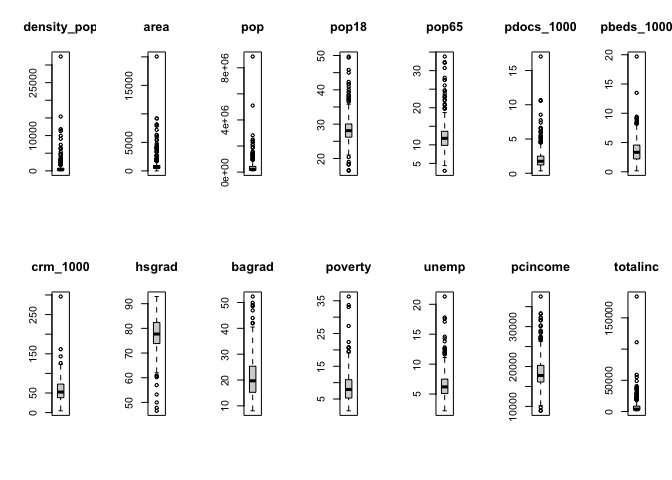
\includegraphics{final_project_files/figure-latex/boxplot-1.pdf}

\hypertarget{correlation}{%
\subsection{Correlation}\label{correlation}}

\hypertarget{pairwise-relationship}{%
\subsubsection{Pairwise relationship}\label{pairwise-relationship}}

\begin{itemize}
\tightlist
\item
  This gives us an idea of the correlation between each variable, but my
  old project build whole model first then assessed the correlation.
  Need Discussion!
\end{itemize}

\begin{Shaded}
\begin{Highlighting}[]
\FunctionTok{library}\NormalTok{(corrplot)}
\end{Highlighting}
\end{Shaded}

\begin{verbatim}
## corrplot 0.92 loaded
\end{verbatim}

\begin{Shaded}
\begin{Highlighting}[]
\FunctionTok{cor}\NormalTok{(cdi\_descriptive) }\SpecialCharTok{\%\textgreater{}\%}\NormalTok{ knitr}\SpecialCharTok{::}\FunctionTok{kable}\NormalTok{()}
\end{Highlighting}
\end{Shaded}

\begin{longtable}[]{@{}
  >{\raggedright\arraybackslash}p{(\columnwidth - 30\tabcolsep) * \real{0.07}}
  >{\raggedleft\arraybackslash}p{(\columnwidth - 30\tabcolsep) * \real{0.06}}
  >{\raggedleft\arraybackslash}p{(\columnwidth - 30\tabcolsep) * \real{0.06}}
  >{\raggedleft\arraybackslash}p{(\columnwidth - 30\tabcolsep) * \real{0.06}}
  >{\raggedleft\arraybackslash}p{(\columnwidth - 30\tabcolsep) * \real{0.06}}
  >{\raggedleft\arraybackslash}p{(\columnwidth - 30\tabcolsep) * \real{0.06}}
  >{\raggedleft\arraybackslash}p{(\columnwidth - 30\tabcolsep) * \real{0.06}}
  >{\raggedleft\arraybackslash}p{(\columnwidth - 30\tabcolsep) * \real{0.06}}
  >{\raggedleft\arraybackslash}p{(\columnwidth - 30\tabcolsep) * \real{0.06}}
  >{\raggedleft\arraybackslash}p{(\columnwidth - 30\tabcolsep) * \real{0.06}}
  >{\raggedleft\arraybackslash}p{(\columnwidth - 30\tabcolsep) * \real{0.06}}
  >{\raggedleft\arraybackslash}p{(\columnwidth - 30\tabcolsep) * \real{0.06}}
  >{\raggedleft\arraybackslash}p{(\columnwidth - 30\tabcolsep) * \real{0.06}}
  >{\raggedleft\arraybackslash}p{(\columnwidth - 30\tabcolsep) * \real{0.06}}
  >{\raggedleft\arraybackslash}p{(\columnwidth - 30\tabcolsep) * \real{0.06}}
  >{\raggedleft\arraybackslash}p{(\columnwidth - 30\tabcolsep) * \real{0.07}}@{}}
\toprule
\begin{minipage}[b]{\linewidth}\raggedright
\end{minipage} & \begin{minipage}[b]{\linewidth}\raggedleft
area
\end{minipage} & \begin{minipage}[b]{\linewidth}\raggedleft
pop
\end{minipage} & \begin{minipage}[b]{\linewidth}\raggedleft
pop18
\end{minipage} & \begin{minipage}[b]{\linewidth}\raggedleft
pop65
\end{minipage} & \begin{minipage}[b]{\linewidth}\raggedleft
crimes
\end{minipage} & \begin{minipage}[b]{\linewidth}\raggedleft
hsgrad
\end{minipage} & \begin{minipage}[b]{\linewidth}\raggedleft
bagrad
\end{minipage} & \begin{minipage}[b]{\linewidth}\raggedleft
poverty
\end{minipage} & \begin{minipage}[b]{\linewidth}\raggedleft
unemp
\end{minipage} & \begin{minipage}[b]{\linewidth}\raggedleft
pcincome
\end{minipage} & \begin{minipage}[b]{\linewidth}\raggedleft
totalinc
\end{minipage} & \begin{minipage}[b]{\linewidth}\raggedleft
crm\_1000
\end{minipage} & \begin{minipage}[b]{\linewidth}\raggedleft
pdocs\_1000
\end{minipage} & \begin{minipage}[b]{\linewidth}\raggedleft
pbeds\_1000
\end{minipage} & \begin{minipage}[b]{\linewidth}\raggedleft
density\_pop
\end{minipage} \\
\midrule
\endhead
area & 1.0000000 & 0.1730834 & -0.0548781 & 0.0057709 & 0.1294754 &
-0.0985981 & -0.1372377 & 0.1713433 & 0.1992093 & -0.1877151 & 0.1270743
& 0.0429484 & -0.1163860 & -0.1412335 & -0.1568156 \\
pop & 0.1730834 & 1.0000000 & 0.0783721 & -0.0290374 & 0.8863318 &
-0.0174269 & 0.1468138 & 0.0380195 & 0.0053517 & 0.2356102 & 0.9867476 &
0.2800992 & 0.1668595 & 0.0203012 & 0.3220266 \\
pop18 & -0.0548781 & 0.0783721 & 1.0000000 & -0.6163096 & 0.0899406 &
0.2505843 & 0.4560970 & 0.0339755 & -0.2785271 & -0.0316484 & 0.0711615
& 0.1905688 & 0.2370280 & 0.0295244 & 0.1254644 \\
pop65 & 0.0057709 & -0.0290374 & -0.6163096 & 1.0000000 & -0.0352903 &
-0.2682518 & -0.3392288 & 0.0065785 & 0.2363094 & 0.0185907 & -0.0227332
& -0.0665333 & 0.0186087 & 0.2471479 & 0.0291845 \\
crimes & 0.1294754 & 0.8863318 & 0.0899406 & -0.0352903 & 1.0000000 &
-0.1063284 & 0.0770765 & 0.1644057 & 0.0435568 & 0.1175391 & 0.8430980 &
0.5300430 & 0.1577103 & 0.0778907 & 0.5609842 \\
hsgrad & -0.0985981 & -0.0174269 & 0.2505843 & -0.2682518 & -0.1063284 &
1.0000000 & 0.7077867 & -0.6917505 & -0.5935958 & 0.5229961 & 0.0433557
& -0.2264129 & 0.1427765 & -0.2111625 & -0.1040070 \\
bagrad & -0.1372377 & 0.1468138 & 0.4560970 & -0.3392288 & 0.0770765 &
0.7077867 & 1.0000000 & -0.4084238 & -0.5409069 & 0.6953619 & 0.2222301
& 0.0383046 & 0.4410463 & -0.0454183 & 0.1556063 \\
poverty & 0.1713433 & 0.0380195 & 0.0339755 & 0.0065785 & 0.1644057 &
-0.6917505 & -0.4084238 & 1.0000000 & 0.4369472 & -0.6017250 &
-0.0387393 & 0.4718442 & 0.0637048 & 0.3713989 & 0.1265079 \\
unemp & 0.1992093 & 0.0053517 & -0.2785271 & 0.2363094 & 0.0435568 &
-0.5935958 & -0.5409069 & 0.4369472 & 1.0000000 & -0.3221444 &
-0.0338763 & 0.0418466 & -0.2478866 & -0.0624878 & 0.0227179 \\
pcincome & -0.1877151 & 0.2356102 & -0.0316484 & 0.0185907 & 0.1175391 &
0.5229961 & 0.6953619 & -0.6017250 & -0.3221444 & 1.0000000 & 0.3476816
& -0.0802442 & 0.3600458 & -0.0535500 & 0.2332260 \\
totalinc & 0.1270743 & 0.9867476 & 0.0711615 & -0.0227332 & 0.8430980 &
0.0433557 & 0.2222301 & -0.0387393 & -0.0338763 & 0.3476816 & 1.0000000
& 0.2281557 & 0.1991038 & 0.0063239 & 0.3162048 \\
crm\_1000 & 0.0429484 & 0.2800992 & 0.1905688 & -0.0665333 & 0.5300430 &
-0.2264129 & 0.0383046 & 0.4718442 & 0.0418466 & -0.0802442 & 0.2281557
& 1.0000000 & 0.3070831 & 0.3644505 & 0.4804285 \\
pdocs\_1000 & -0.1163860 & 0.1668595 & 0.2370280 & 0.0186087 & 0.1577103
& 0.1427765 & 0.4410463 & 0.0637048 & -0.2478866 & 0.3600458 & 0.1991038
& 0.3070831 & 1.0000000 & 0.6666947 & 0.3180424 \\
pbeds\_1000 & -0.1412335 & 0.0203012 & 0.0295244 & 0.2471479 & 0.0778907
& -0.2111625 & -0.0454183 & 0.3713989 & -0.0624878 & -0.0535500 &
0.0063239 & 0.3644505 & 0.6666947 & 1.0000000 & 0.2064177 \\
density\_pop & -0.1568156 & 0.3220266 & 0.1254644 & 0.0291845 &
0.5609842 & -0.1040070 & 0.1556063 & 0.1265079 & 0.0227179 & 0.2332260 &
0.3162048 & 0.4804285 & 0.3180424 & 0.2064177 & 1.0000000 \\
\bottomrule
\end{longtable}

\begin{Shaded}
\begin{Highlighting}[]
\FunctionTok{library}\NormalTok{(ggcorrplot)}

\FunctionTok{ggcorrplot}\NormalTok{(}\FunctionTok{cor}\NormalTok{(cdi\_descriptive), }\AttributeTok{type =} \StringTok{"upper"}\NormalTok{,}
   \AttributeTok{lab =} \ConstantTok{TRUE}\NormalTok{)}
\end{Highlighting}
\end{Shaded}

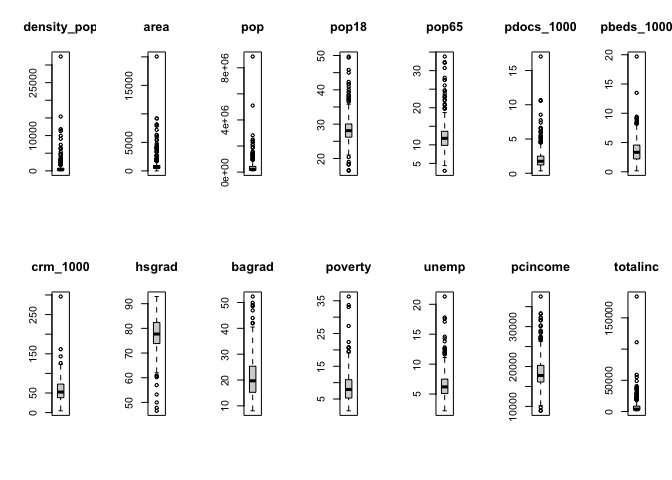
\includegraphics{final_project_files/figure-latex/unnamed-chunk-2-1.pdf}

Scatter plot

\begin{Shaded}
\begin{Highlighting}[]
\FunctionTok{pairs}\NormalTok{(crm\_1000 }\SpecialCharTok{\textasciitilde{}}\NormalTok{.,}\AttributeTok{data=}\NormalTok{cdi\_descriptive, }\AttributeTok{panel =}\NormalTok{ panel.smooth, }\AttributeTok{upper.panel =} \ConstantTok{NULL}\NormalTok{, }\AttributeTok{main =} \StringTok{"Scatterplot Matrix"}\NormalTok{)}
\end{Highlighting}
\end{Shaded}

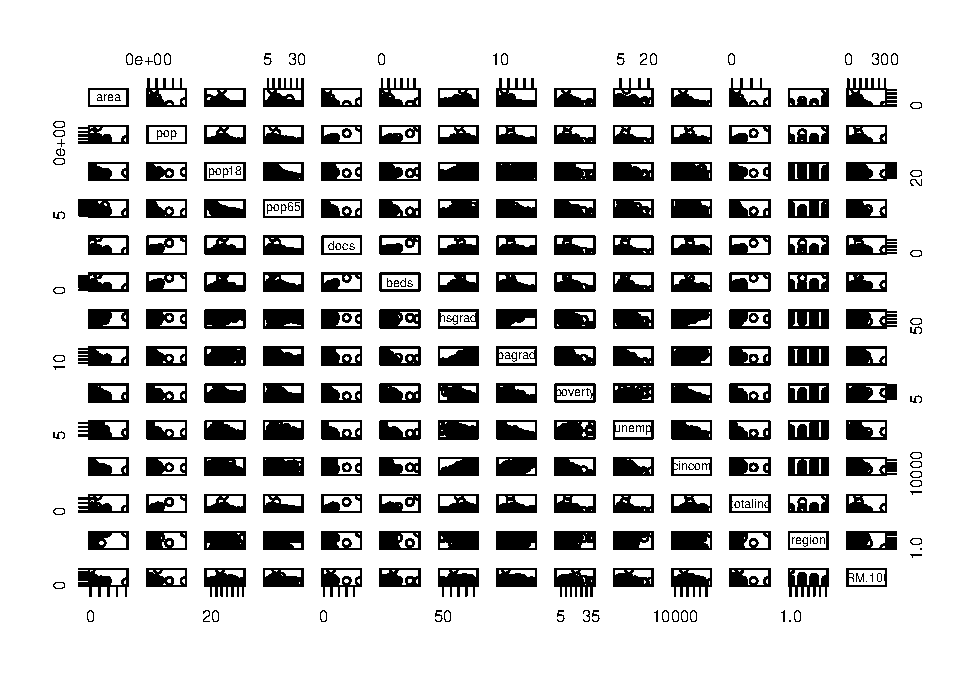
\includegraphics{final_project_files/figure-latex/unnamed-chunk-3-1.pdf}

\hypertarget{marginal-distribution}{%
\subsection{Marginal distribution}\label{marginal-distribution}}

\begin{Shaded}
\begin{Highlighting}[]
\FunctionTok{library}\NormalTok{(ggplot2)}
\FunctionTok{library}\NormalTok{(ggExtra)}
\end{Highlighting}
\end{Shaded}

\begin{Shaded}
\begin{Highlighting}[]
\NormalTok{marg\_den }\OtherTok{=}\NormalTok{ cdi }\SpecialCharTok{\%\textgreater{}\%} \FunctionTok{ggplot}\NormalTok{(}\FunctionTok{aes}\NormalTok{(}\AttributeTok{x =}\NormalTok{ density\_pop, }\AttributeTok{y =}\NormalTok{ crm\_1000)) }\SpecialCharTok{+} \FunctionTok{geom\_point}\NormalTok{(}\AttributeTok{alpha =} \FloatTok{0.3}\NormalTok{) }\SpecialCharTok{+} \FunctionTok{geom\_smooth}\NormalTok{(}\AttributeTok{method =} \StringTok{\textquotesingle{}lm\textquotesingle{}}\NormalTok{, }\AttributeTok{se =} \ConstantTok{TRUE}\NormalTok{, }\AttributeTok{color =} \StringTok{\textquotesingle{}red\textquotesingle{}}\NormalTok{)}
\FunctionTok{ggMarginal}\NormalTok{(marg\_den, }\AttributeTok{type =} \StringTok{"histogram"}\NormalTok{, }\AttributeTok{fill=}\StringTok{"transparent"}\NormalTok{)}
\end{Highlighting}
\end{Shaded}

\begin{verbatim}
## `geom_smooth()` using formula 'y ~ x'
## `geom_smooth()` using formula 'y ~ x'
\end{verbatim}

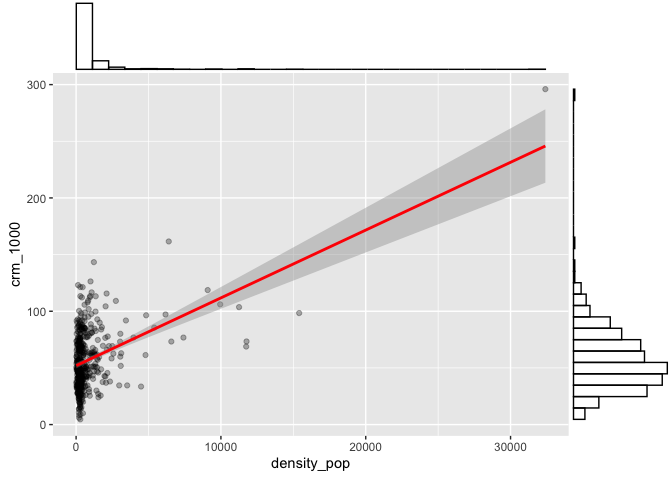
\includegraphics{final_project_files/figure-latex/unnamed-chunk-5-1.pdf}

\begin{Shaded}
\begin{Highlighting}[]
\NormalTok{marg\_area }\OtherTok{=}\NormalTok{ cdi }\SpecialCharTok{\%\textgreater{}\%} \FunctionTok{ggplot}\NormalTok{(}\FunctionTok{aes}\NormalTok{(}\AttributeTok{x =}\NormalTok{ area, }\AttributeTok{y =}\NormalTok{ crm\_1000)) }\SpecialCharTok{+} \FunctionTok{geom\_point}\NormalTok{(}\AttributeTok{alpha =} \FloatTok{0.3}\NormalTok{) }\SpecialCharTok{+} \FunctionTok{geom\_smooth}\NormalTok{(}\AttributeTok{method =} \StringTok{\textquotesingle{}lm\textquotesingle{}}\NormalTok{, }\AttributeTok{se =} \ConstantTok{TRUE}\NormalTok{, }\AttributeTok{color =} \StringTok{\textquotesingle{}red\textquotesingle{}}\NormalTok{)}
\FunctionTok{ggMarginal}\NormalTok{(marg\_area, }\AttributeTok{type =} \StringTok{"histogram"}\NormalTok{, }\AttributeTok{fill=}\StringTok{"transparent"}\NormalTok{)}
\end{Highlighting}
\end{Shaded}

\begin{verbatim}
## `geom_smooth()` using formula 'y ~ x'
## `geom_smooth()` using formula 'y ~ x'
\end{verbatim}

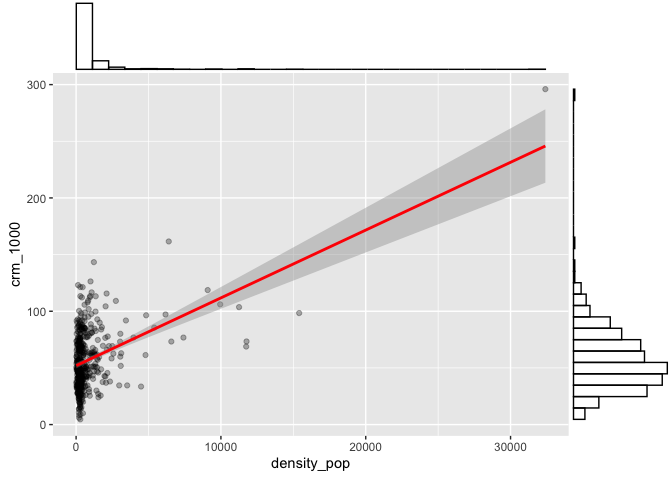
\includegraphics{final_project_files/figure-latex/unnamed-chunk-6-1.pdf}

\begin{Shaded}
\begin{Highlighting}[]
\NormalTok{marg\_pop }\OtherTok{=}\NormalTok{ cdi }\SpecialCharTok{\%\textgreater{}\%} \FunctionTok{ggplot}\NormalTok{(}\FunctionTok{aes}\NormalTok{(}\AttributeTok{x =}\NormalTok{ pop, }\AttributeTok{y =}\NormalTok{ crm\_1000)) }\SpecialCharTok{+} \FunctionTok{geom\_point}\NormalTok{(}\AttributeTok{alpha =} \FloatTok{0.3}\NormalTok{) }\SpecialCharTok{+} \FunctionTok{geom\_smooth}\NormalTok{(}\AttributeTok{method =} \StringTok{\textquotesingle{}lm\textquotesingle{}}\NormalTok{, }\AttributeTok{se =} \ConstantTok{TRUE}\NormalTok{, }\AttributeTok{color =} \StringTok{\textquotesingle{}red\textquotesingle{}}\NormalTok{)}
\FunctionTok{ggMarginal}\NormalTok{(marg\_pop, }\AttributeTok{type =} \StringTok{"histogram"}\NormalTok{, }\AttributeTok{fill=}\StringTok{"transparent"}\NormalTok{)}
\end{Highlighting}
\end{Shaded}

\begin{verbatim}
## `geom_smooth()` using formula 'y ~ x'
## `geom_smooth()` using formula 'y ~ x'
\end{verbatim}

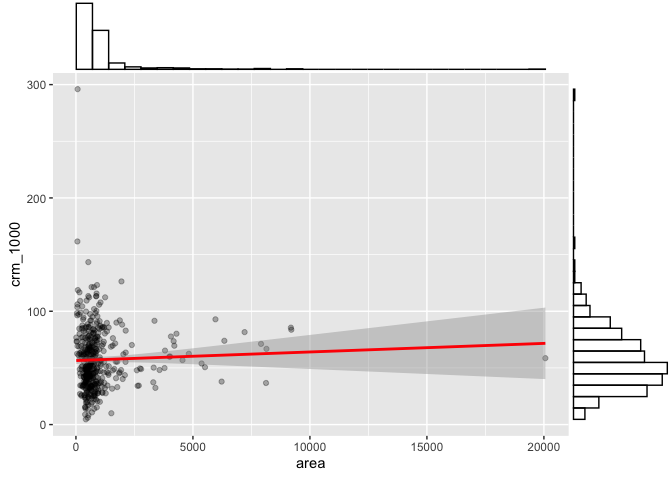
\includegraphics{final_project_files/figure-latex/unnamed-chunk-7-1.pdf}

\begin{Shaded}
\begin{Highlighting}[]
\NormalTok{marg\_pop18 }\OtherTok{=}\NormalTok{ cdi }\SpecialCharTok{\%\textgreater{}\%} \FunctionTok{ggplot}\NormalTok{(}\FunctionTok{aes}\NormalTok{(}\AttributeTok{x =}\NormalTok{ pop18, }\AttributeTok{y =}\NormalTok{ crm\_1000)) }\SpecialCharTok{+} \FunctionTok{geom\_point}\NormalTok{(}\AttributeTok{alpha =} \FloatTok{0.3}\NormalTok{) }\SpecialCharTok{+} \FunctionTok{geom\_smooth}\NormalTok{(}\AttributeTok{method =} \StringTok{\textquotesingle{}lm\textquotesingle{}}\NormalTok{, }\AttributeTok{se =} \ConstantTok{TRUE}\NormalTok{, }\AttributeTok{color =} \StringTok{\textquotesingle{}red\textquotesingle{}}\NormalTok{)}
\CommentTok{\# positive correlation}
\FunctionTok{ggMarginal}\NormalTok{(marg\_pop18, }\AttributeTok{type =} \StringTok{"histogram"}\NormalTok{, }\AttributeTok{fill=}\StringTok{"transparent"}\NormalTok{)}
\end{Highlighting}
\end{Shaded}

\begin{verbatim}
## `geom_smooth()` using formula 'y ~ x'
## `geom_smooth()` using formula 'y ~ x'
\end{verbatim}

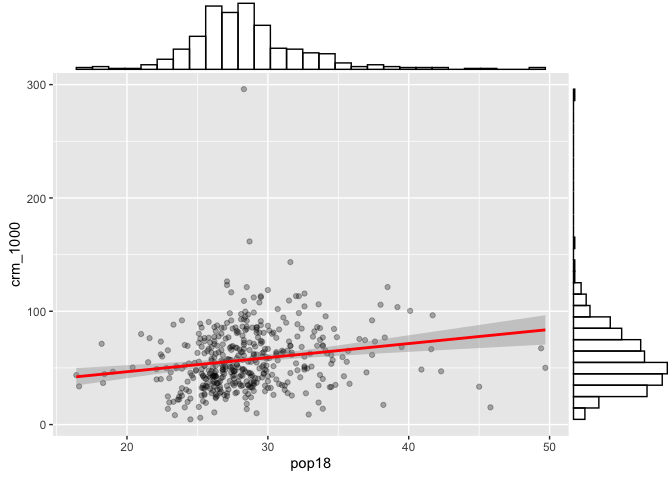
\includegraphics{final_project_files/figure-latex/unnamed-chunk-8-1.pdf}

\begin{Shaded}
\begin{Highlighting}[]
\NormalTok{marg\_pop65 }\OtherTok{=}\NormalTok{ cdi }\SpecialCharTok{\%\textgreater{}\%} \FunctionTok{ggplot}\NormalTok{(}\FunctionTok{aes}\NormalTok{(}\AttributeTok{x =}\NormalTok{ pop65, }\AttributeTok{y =}\NormalTok{ crm\_1000)) }\SpecialCharTok{+} \FunctionTok{geom\_point}\NormalTok{(}\AttributeTok{alpha =} \FloatTok{0.3}\NormalTok{) }\SpecialCharTok{+} \FunctionTok{geom\_smooth}\NormalTok{(}\AttributeTok{method =} \StringTok{\textquotesingle{}lm\textquotesingle{}}\NormalTok{, }\AttributeTok{se =} \ConstantTok{TRUE}\NormalTok{, }\AttributeTok{color =} \StringTok{\textquotesingle{}red\textquotesingle{}}\NormalTok{)}
\FunctionTok{ggMarginal}\NormalTok{(marg\_pop65, }\AttributeTok{type =} \StringTok{"histogram"}\NormalTok{, }\AttributeTok{fill=}\StringTok{"transparent"}\NormalTok{)}
\end{Highlighting}
\end{Shaded}

\begin{verbatim}
## `geom_smooth()` using formula 'y ~ x'
## `geom_smooth()` using formula 'y ~ x'
\end{verbatim}

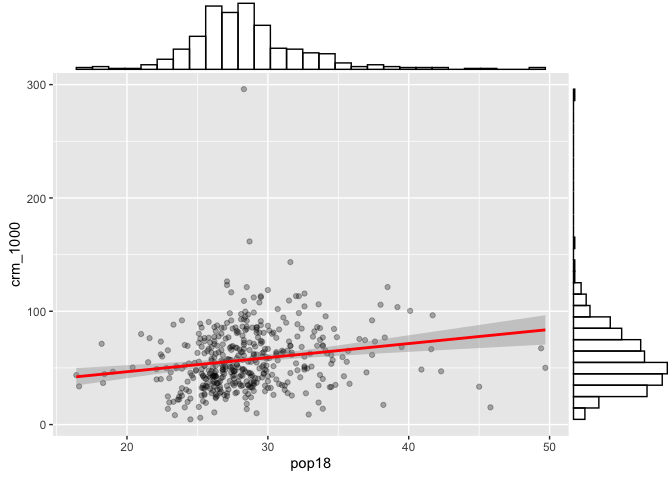
\includegraphics{final_project_files/figure-latex/unnamed-chunk-9-1.pdf}

\begin{Shaded}
\begin{Highlighting}[]
\NormalTok{marg\_pdocs\_1000 }\OtherTok{=}\NormalTok{ cdi }\SpecialCharTok{\%\textgreater{}\%} \FunctionTok{ggplot}\NormalTok{(}\FunctionTok{aes}\NormalTok{(}\AttributeTok{x =}\NormalTok{ pdocs\_1000, }\AttributeTok{y =}\NormalTok{ crm\_1000)) }\SpecialCharTok{+} \FunctionTok{geom\_point}\NormalTok{(}\AttributeTok{alpha =} \FloatTok{0.3}\NormalTok{) }\SpecialCharTok{+} \FunctionTok{geom\_smooth}\NormalTok{(}\AttributeTok{method =} \StringTok{\textquotesingle{}lm\textquotesingle{}}\NormalTok{, }\AttributeTok{se =} \ConstantTok{TRUE}\NormalTok{, }\AttributeTok{color =} \StringTok{\textquotesingle{}red\textquotesingle{}}\NormalTok{)}
\FunctionTok{ggMarginal}\NormalTok{(marg\_pdocs\_1000, }\AttributeTok{type =} \StringTok{"histogram"}\NormalTok{, }\AttributeTok{fill=}\StringTok{"transparent"}\NormalTok{)}
\end{Highlighting}
\end{Shaded}

\begin{verbatim}
## `geom_smooth()` using formula 'y ~ x'
## `geom_smooth()` using formula 'y ~ x'
\end{verbatim}

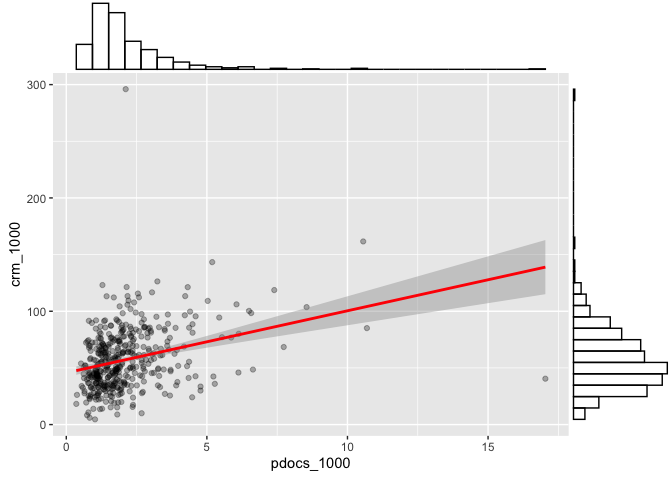
\includegraphics{final_project_files/figure-latex/unnamed-chunk-10-1.pdf}

\begin{Shaded}
\begin{Highlighting}[]
\NormalTok{marg\_pbeds\_1000 }\OtherTok{=}\NormalTok{ cdi }\SpecialCharTok{\%\textgreater{}\%} \FunctionTok{ggplot}\NormalTok{(}\FunctionTok{aes}\NormalTok{(}\AttributeTok{x =}\NormalTok{ pbeds\_1000, }\AttributeTok{y =}\NormalTok{ crm\_1000)) }\SpecialCharTok{+} \FunctionTok{geom\_point}\NormalTok{(}\AttributeTok{alpha =} \FloatTok{0.3}\NormalTok{) }\SpecialCharTok{+} \FunctionTok{geom\_smooth}\NormalTok{(}\AttributeTok{method =} \StringTok{\textquotesingle{}lm\textquotesingle{}}\NormalTok{, }\AttributeTok{se =} \ConstantTok{TRUE}\NormalTok{, }\AttributeTok{color =} \StringTok{\textquotesingle{}red\textquotesingle{}}\NormalTok{)}
\FunctionTok{ggMarginal}\NormalTok{(marg\_pbeds\_1000, }\AttributeTok{type =} \StringTok{"histogram"}\NormalTok{, }\AttributeTok{fill=}\StringTok{"transparent"}\NormalTok{)}
\end{Highlighting}
\end{Shaded}

\begin{verbatim}
## `geom_smooth()` using formula 'y ~ x'
## `geom_smooth()` using formula 'y ~ x'
\end{verbatim}

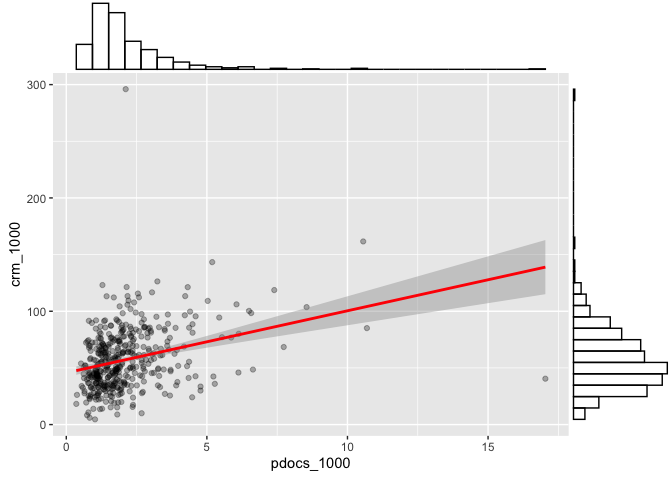
\includegraphics{final_project_files/figure-latex/unnamed-chunk-11-1.pdf}

\begin{Shaded}
\begin{Highlighting}[]
\NormalTok{marg\_hsgrad }\OtherTok{=}\NormalTok{ cdi }\SpecialCharTok{\%\textgreater{}\%} \FunctionTok{ggplot}\NormalTok{(}\FunctionTok{aes}\NormalTok{(}\AttributeTok{x =}\NormalTok{ hsgrad, }\AttributeTok{y =}\NormalTok{ crm\_1000)) }\SpecialCharTok{+} \FunctionTok{geom\_point}\NormalTok{(}\AttributeTok{alpha =} \FloatTok{0.3}\NormalTok{) }\SpecialCharTok{+} \FunctionTok{geom\_smooth}\NormalTok{(}\AttributeTok{method =} \StringTok{\textquotesingle{}lm\textquotesingle{}}\NormalTok{, }\AttributeTok{se =} \ConstantTok{TRUE}\NormalTok{, }\AttributeTok{color =} \StringTok{\textquotesingle{}red\textquotesingle{}}\NormalTok{) }\CommentTok{\#negative correlation}
\FunctionTok{ggMarginal}\NormalTok{(marg\_hsgrad, }\AttributeTok{type =} \StringTok{"histogram"}\NormalTok{, }\AttributeTok{fill=}\StringTok{"transparent"}\NormalTok{)}
\end{Highlighting}
\end{Shaded}

\begin{verbatim}
## `geom_smooth()` using formula 'y ~ x'
## `geom_smooth()` using formula 'y ~ x'
\end{verbatim}

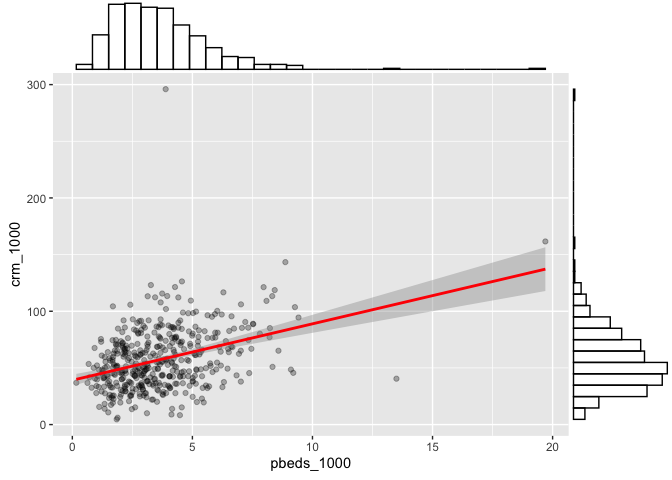
\includegraphics{final_project_files/figure-latex/unnamed-chunk-12-1.pdf}

\begin{Shaded}
\begin{Highlighting}[]
\NormalTok{marg\_bagrad }\OtherTok{=}\NormalTok{ cdi }\SpecialCharTok{\%\textgreater{}\%} \FunctionTok{ggplot}\NormalTok{(}\FunctionTok{aes}\NormalTok{(}\AttributeTok{x =}\NormalTok{ bagrad, }\AttributeTok{y =}\NormalTok{ crm\_1000)) }\SpecialCharTok{+} \FunctionTok{geom\_point}\NormalTok{(}\AttributeTok{alpha =} \FloatTok{0.3}\NormalTok{) }\SpecialCharTok{+} \FunctionTok{geom\_smooth}\NormalTok{(}\AttributeTok{method =} \StringTok{\textquotesingle{}lm\textquotesingle{}}\NormalTok{, }\AttributeTok{se =} \ConstantTok{TRUE}\NormalTok{, }\AttributeTok{color =} \StringTok{\textquotesingle{}red\textquotesingle{}}\NormalTok{)}
\FunctionTok{ggMarginal}\NormalTok{(marg\_bagrad, }\AttributeTok{type =} \StringTok{"histogram"}\NormalTok{, }\AttributeTok{fill=}\StringTok{"transparent"}\NormalTok{)}
\end{Highlighting}
\end{Shaded}

\begin{verbatim}
## `geom_smooth()` using formula 'y ~ x'
## `geom_smooth()` using formula 'y ~ x'
\end{verbatim}

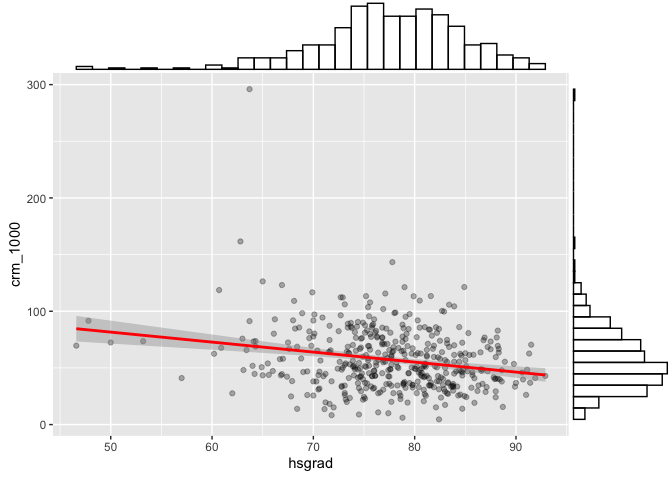
\includegraphics{final_project_files/figure-latex/unnamed-chunk-13-1.pdf}

\begin{Shaded}
\begin{Highlighting}[]
\NormalTok{marg\_poverty }\OtherTok{=}\NormalTok{ cdi }\SpecialCharTok{\%\textgreater{}\%} \FunctionTok{ggplot}\NormalTok{(}\FunctionTok{aes}\NormalTok{(}\AttributeTok{x =}\NormalTok{ poverty, }\AttributeTok{y =}\NormalTok{ crm\_1000)) }\SpecialCharTok{+} \FunctionTok{geom\_point}\NormalTok{(}\AttributeTok{alpha =} \FloatTok{0.3}\NormalTok{) }\SpecialCharTok{+} \FunctionTok{geom\_smooth}\NormalTok{(}\AttributeTok{method =} \StringTok{\textquotesingle{}lm\textquotesingle{}}\NormalTok{, }\AttributeTok{se =} \ConstantTok{TRUE}\NormalTok{, }\AttributeTok{color =} \StringTok{\textquotesingle{}red\textquotesingle{}}\NormalTok{) }\CommentTok{\# positive correlation}
\FunctionTok{ggMarginal}\NormalTok{(marg\_poverty, }\AttributeTok{type =} \StringTok{"histogram"}\NormalTok{, }\AttributeTok{fill=}\StringTok{"transparent"}\NormalTok{)}
\end{Highlighting}
\end{Shaded}

\begin{verbatim}
## `geom_smooth()` using formula 'y ~ x'
## `geom_smooth()` using formula 'y ~ x'
\end{verbatim}

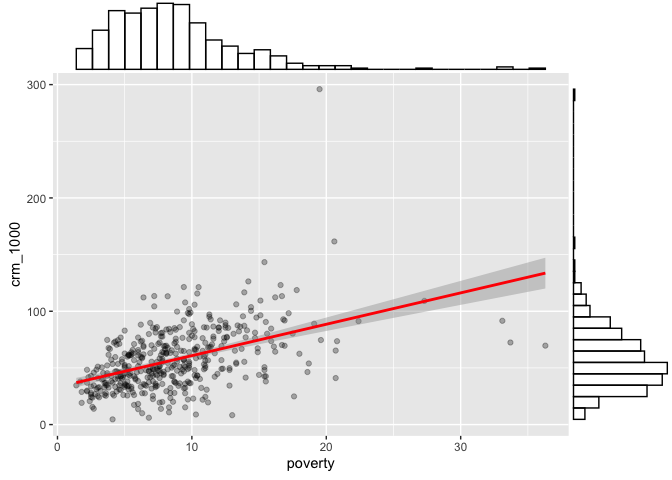
\includegraphics{final_project_files/figure-latex/unnamed-chunk-14-1.pdf}

\begin{Shaded}
\begin{Highlighting}[]
\NormalTok{marg\_unemp }\OtherTok{=}\NormalTok{ cdi }\SpecialCharTok{\%\textgreater{}\%} \FunctionTok{ggplot}\NormalTok{(}\FunctionTok{aes}\NormalTok{(}\AttributeTok{x =}\NormalTok{ unemp, }\AttributeTok{y =}\NormalTok{ crm\_1000)) }\SpecialCharTok{+} \FunctionTok{geom\_point}\NormalTok{(}\AttributeTok{alpha =} \FloatTok{0.3}\NormalTok{) }\SpecialCharTok{+} \FunctionTok{geom\_smooth}\NormalTok{(}\AttributeTok{method =} \StringTok{\textquotesingle{}lm\textquotesingle{}}\NormalTok{, }\AttributeTok{se =} \ConstantTok{TRUE}\NormalTok{, }\AttributeTok{color =} \StringTok{\textquotesingle{}red\textquotesingle{}}\NormalTok{)}
\FunctionTok{ggMarginal}\NormalTok{(marg\_unemp, }\AttributeTok{type =} \StringTok{"histogram"}\NormalTok{, }\AttributeTok{fill=}\StringTok{"transparent"}\NormalTok{)}
\end{Highlighting}
\end{Shaded}

\begin{verbatim}
## `geom_smooth()` using formula 'y ~ x'
## `geom_smooth()` using formula 'y ~ x'
\end{verbatim}

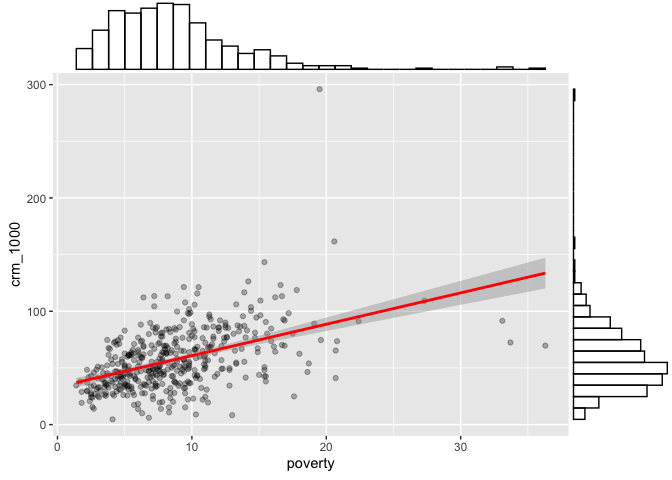
\includegraphics{final_project_files/figure-latex/unnamed-chunk-15-1.pdf}

\begin{Shaded}
\begin{Highlighting}[]
\NormalTok{marg\_pcincome }\OtherTok{=}\NormalTok{ cdi }\SpecialCharTok{\%\textgreater{}\%} \FunctionTok{ggplot}\NormalTok{(}\FunctionTok{aes}\NormalTok{(}\AttributeTok{x =}\NormalTok{ pcincome, }\AttributeTok{y =}\NormalTok{ crm\_1000)) }\SpecialCharTok{+} \FunctionTok{geom\_point}\NormalTok{(}\AttributeTok{alpha =} \FloatTok{0.3}\NormalTok{) }\SpecialCharTok{+} \FunctionTok{geom\_smooth}\NormalTok{(}\AttributeTok{method =} \StringTok{\textquotesingle{}lm\textquotesingle{}}\NormalTok{, }\AttributeTok{se =} \ConstantTok{TRUE}\NormalTok{, }\AttributeTok{color =} \StringTok{\textquotesingle{}red\textquotesingle{}}\NormalTok{)}
\FunctionTok{ggMarginal}\NormalTok{(marg\_pcincome, }\AttributeTok{type =} \StringTok{"histogram"}\NormalTok{, }\AttributeTok{fill=}\StringTok{"transparent"}\NormalTok{)}
\end{Highlighting}
\end{Shaded}

\begin{verbatim}
## `geom_smooth()` using formula 'y ~ x'
## `geom_smooth()` using formula 'y ~ x'
\end{verbatim}

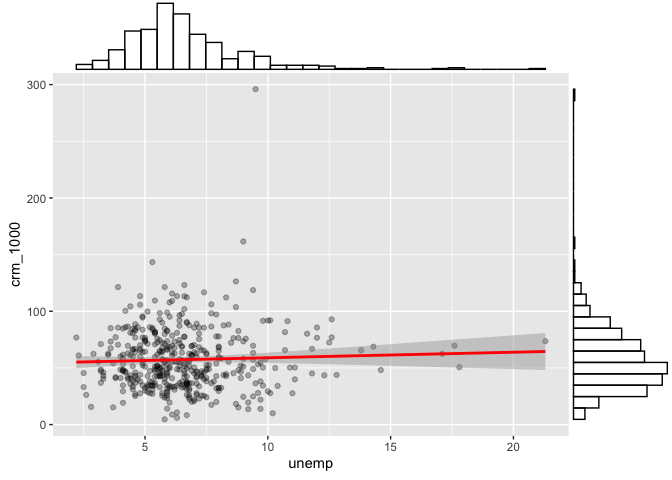
\includegraphics{final_project_files/figure-latex/unnamed-chunk-16-1.pdf}

\begin{Shaded}
\begin{Highlighting}[]
\NormalTok{marg\_totalinc }\OtherTok{=}\NormalTok{ cdi }\SpecialCharTok{\%\textgreater{}\%} \FunctionTok{ggplot}\NormalTok{(}\FunctionTok{aes}\NormalTok{(}\AttributeTok{x =}\NormalTok{ totalinc, }\AttributeTok{y =}\NormalTok{ crm\_1000)) }\SpecialCharTok{+} \FunctionTok{geom\_point}\NormalTok{(}\AttributeTok{alpha =} \FloatTok{0.3}\NormalTok{) }\SpecialCharTok{+} \FunctionTok{geom\_smooth}\NormalTok{(}\AttributeTok{method =} \StringTok{\textquotesingle{}lm\textquotesingle{}}\NormalTok{, }\AttributeTok{se =} \ConstantTok{TRUE}\NormalTok{, }\AttributeTok{color =} \StringTok{\textquotesingle{}red\textquotesingle{}}\NormalTok{)}
\FunctionTok{ggMarginal}\NormalTok{(marg\_totalinc, }\AttributeTok{type =} \StringTok{"histogram"}\NormalTok{, }\AttributeTok{fill=}\StringTok{"transparent"}\NormalTok{)}
\end{Highlighting}
\end{Shaded}

\begin{verbatim}
## `geom_smooth()` using formula 'y ~ x'
## `geom_smooth()` using formula 'y ~ x'
\end{verbatim}

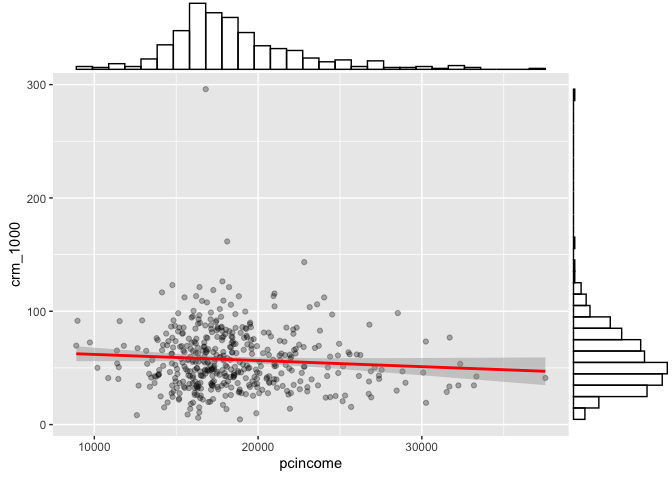
\includegraphics{final_project_files/figure-latex/unnamed-chunk-17-1.pdf}

\hypertarget{distribution-of-outcome}{%
\subsection{Distribution of outcome}\label{distribution-of-outcome}}

\begin{Shaded}
\begin{Highlighting}[]
\NormalTok{cdi }\SpecialCharTok{\%\textgreater{}\%} 
  \FunctionTok{ggplot}\NormalTok{(}\FunctionTok{aes}\NormalTok{(}\AttributeTok{x =}\NormalTok{ crm\_1000)) }\SpecialCharTok{+}
  \FunctionTok{geom\_histogram}\NormalTok{()}
\end{Highlighting}
\end{Shaded}

\begin{verbatim}
## `stat_bin()` using `bins = 30`. Pick better value with `binwidth`.
\end{verbatim}

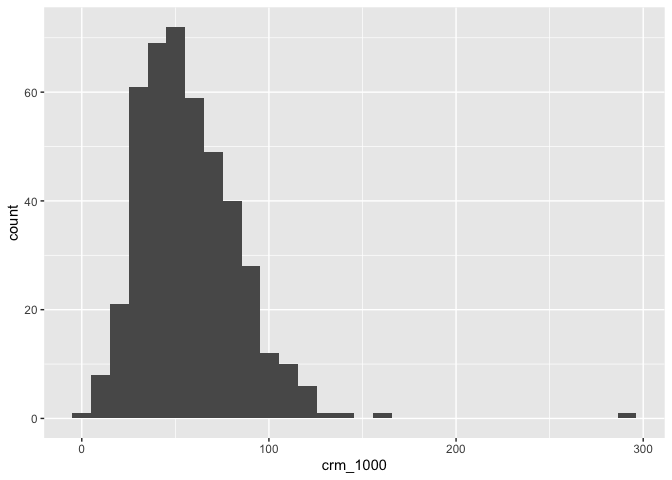
\includegraphics{final_project_files/figure-latex/unnamed-chunk-18-1.pdf}

do we look at the distribution of outcome like this and transform them
here? check again

\hypertarget{counties-with-unusual-rates}{%
\subsection{Counties with unusual
rates}\label{counties-with-unusual-rates}}

\begin{Shaded}
\begin{Highlighting}[]
\NormalTok{upper }\OtherTok{=} \FunctionTok{quantile}\NormalTok{(cdi}\SpecialCharTok{$}\NormalTok{crm\_1000, }\FloatTok{0.75}\NormalTok{)}
\NormalTok{lower }\OtherTok{=} \FunctionTok{quantile}\NormalTok{(cdi}\SpecialCharTok{$}\NormalTok{crm\_1000, }\FloatTok{0.25}\NormalTok{)}
\NormalTok{IQR }\OtherTok{=}\NormalTok{ upper }\SpecialCharTok{{-}}\NormalTok{ lower}
\NormalTok{cdi }\SpecialCharTok{\%\textgreater{}\%} 
  \FunctionTok{filter}\NormalTok{(crm\_1000 }\SpecialCharTok{\textgreater{}}\NormalTok{ upper }\SpecialCharTok{+} \FloatTok{1.5}\SpecialCharTok{*}\NormalTok{IQR,}
\NormalTok{         crm\_1000 }\SpecialCharTok{\textgreater{}}\NormalTok{ lower }\SpecialCharTok{{-}} \FloatTok{1.5}\SpecialCharTok{*}\NormalTok{IQR) }\SpecialCharTok{\%\textgreater{}\%} 
\NormalTok{  dplyr}\SpecialCharTok{::}\FunctionTok{select}\NormalTok{(cty, crm\_1000) }\SpecialCharTok{\%\textgreater{}\%}
\NormalTok{  knitr}\SpecialCharTok{::}\FunctionTok{kable}\NormalTok{(}\AttributeTok{digits =} \DecValTok{2}\NormalTok{)}
\end{Highlighting}
\end{Shaded}

\begin{longtable}[]{@{}lr@{}}
\toprule
cty & crm\_1000 \\
\midrule
\endhead
Kings & 295.99 \\
Dade & 126.34 \\
Fulton & 143.35 \\
St.\_Loui & 161.60 \\
\bottomrule
\end{longtable}

\hypertarget{model}{%
\section{Model}\label{model}}

\hypertarget{full-model-predictors}{%
\subsection{Full model predictors}\label{full-model-predictors}}

this model used \texttt{northeast} as the reference level for region

\begin{Shaded}
\begin{Highlighting}[]
\NormalTok{cdi\_model }\OtherTok{=}\NormalTok{ cdi }\SpecialCharTok{\%\textgreater{}\%} \FunctionTok{select}\NormalTok{(}\SpecialCharTok{{-}}\FunctionTok{c}\NormalTok{(id,cty,state,area,crimes,totalinc))}

\CommentTok{\# use }
\NormalTok{full\_fit }\OtherTok{=} \FunctionTok{lm}\NormalTok{(crm\_1000 }\SpecialCharTok{\textasciitilde{}}\NormalTok{ ., }\AttributeTok{data =}\NormalTok{ cdi\_model)}
\FunctionTok{summary}\NormalTok{(full\_fit)}
\end{Highlighting}
\end{Shaded}

\begin{verbatim}
## 
## Call:
## lm(formula = crm_1000 ~ ., data = cdi_model)
## 
## Residuals:
##     Min      1Q  Median      3Q     Max 
## -47.786 -11.422  -0.934  10.200  75.180 
## 
## Coefficients:
##                      Estimate Std. Error t value Pr(>|t|)    
## (Intercept)        -6.922e+01  2.739e+01  -2.528 0.011849 *  
## pop                 5.486e-06  1.579e-06   3.474 0.000566 ***
## pop18               6.947e-01  3.305e-01   2.102 0.036150 *  
## pop65              -1.998e-01  3.055e-01  -0.654 0.513410    
## hsgrad              6.143e-01  2.690e-01   2.284 0.022864 *  
## bagrad             -4.835e-01  2.971e-01  -1.628 0.104327    
## poverty             1.856e+00  3.864e-01   4.803 2.17e-06 ***
## unemp               6.111e-01  5.314e-01   1.150 0.250812    
## pcincome            1.039e-03  4.734e-04   2.195 0.028670 *  
## regionnorthcentral  8.978e+00  2.732e+00   3.286 0.001100 ** 
## regionsouth         2.779e+01  2.659e+00  10.453  < 2e-16 ***
## regionwest          2.118e+01  3.125e+00   6.778 4.09e-11 ***
## pdocs_1000         -6.634e-01  1.019e+00  -0.651 0.515556    
## pbeds_1000          3.157e+00  7.939e-01   3.977 8.21e-05 ***
## density_pop         4.901e-03  4.537e-04  10.802  < 2e-16 ***
## ---
## Signif. codes:  0 '***' 0.001 '**' 0.01 '*' 0.05 '.' 0.1 ' ' 1
## 
## Residual standard error: 17.81 on 425 degrees of freedom
## Multiple R-squared:  0.589,  Adjusted R-squared:  0.5755 
## F-statistic: 43.51 on 14 and 425 DF,  p-value: < 2.2e-16
\end{verbatim}

\begin{Shaded}
\begin{Highlighting}[]
\NormalTok{olsrr}\SpecialCharTok{::}\FunctionTok{ols\_plot\_resid\_qq}\NormalTok{(full\_fit)}
\end{Highlighting}
\end{Shaded}

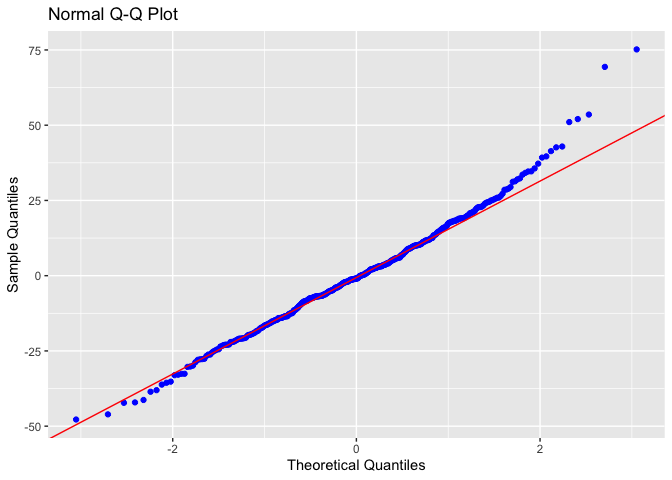
\includegraphics{final_project_files/figure-latex/unnamed-chunk-20-1.pdf}

\begin{Shaded}
\begin{Highlighting}[]
\NormalTok{olsrr}\SpecialCharTok{::}\FunctionTok{ols\_plot\_resid\_fit}\NormalTok{(full\_fit)}
\end{Highlighting}
\end{Shaded}

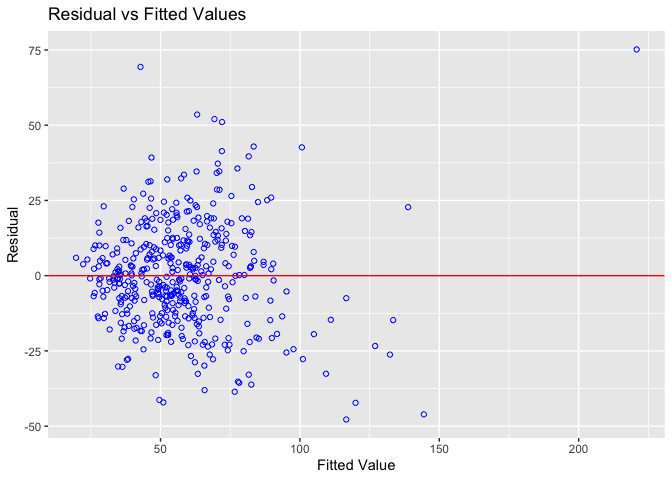
\includegraphics{final_project_files/figure-latex/unnamed-chunk-20-2.pdf}

\hypertarget{transformation}{%
\subsection{Transformation}\label{transformation}}

\begin{Shaded}
\begin{Highlighting}[]
\NormalTok{lambda }\OtherTok{=}\NormalTok{ MASS}\SpecialCharTok{::}\FunctionTok{boxcox}\NormalTok{(full\_fit)}
\end{Highlighting}
\end{Shaded}

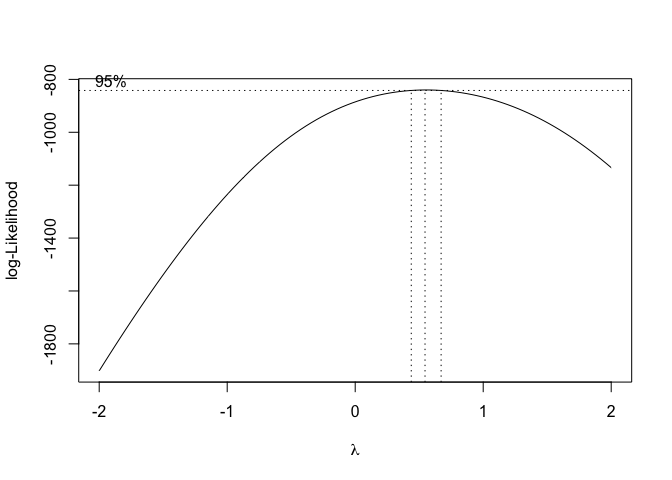
\includegraphics{final_project_files/figure-latex/unnamed-chunk-21-1.pdf}

\begin{Shaded}
\begin{Highlighting}[]
\NormalTok{optlam }\OtherTok{=}\NormalTok{ lambda}\SpecialCharTok{$}\NormalTok{x[}\FunctionTok{which.max}\NormalTok{(lambda}\SpecialCharTok{$}\NormalTok{y)]}
\NormalTok{optlam}
\end{Highlighting}
\end{Shaded}

\begin{verbatim}
## [1] 0.5454545
\end{verbatim}

The lambda from the transformation is 0.5454, so we will try to fit a
square root transformation to Y

New tibble with transformed Y:

\begin{Shaded}
\begin{Highlighting}[]
\NormalTok{cdi\_trans }\OtherTok{=}\NormalTok{ cdi\_model }\SpecialCharTok{\%\textgreater{}\%} \FunctionTok{mutate}\NormalTok{(}\AttributeTok{crm\_1000\_sqr =}\NormalTok{ crm\_1000}\SpecialCharTok{\^{}}\FloatTok{0.5}\NormalTok{) }\SpecialCharTok{\%\textgreater{}\%} \FunctionTok{select}\NormalTok{(}\SpecialCharTok{{-}}\FunctionTok{c}\NormalTok{(crm\_1000))}
\end{Highlighting}
\end{Shaded}

\begin{Shaded}
\begin{Highlighting}[]
\NormalTok{trans\_fit }\OtherTok{=} \FunctionTok{lm}\NormalTok{(crm\_1000\_sqr }\SpecialCharTok{\textasciitilde{}}\NormalTok{ .,}\AttributeTok{data =}\NormalTok{ cdi\_trans)}
\FunctionTok{summary}\NormalTok{(trans\_fit)}
\end{Highlighting}
\end{Shaded}

\begin{verbatim}
## 
## Call:
## lm(formula = crm_1000_sqr ~ ., data = cdi_trans)
## 
## Residuals:
##     Min      1Q  Median      3Q     Max 
## -4.0410 -0.7300  0.0708  0.7485  4.0273 
## 
## Coefficients:
##                      Estimate Std. Error t value Pr(>|t|)    
## (Intercept)        -1.645e+00  1.802e+00  -0.913 0.361766    
## pop                 3.624e-07  1.039e-07   3.488 0.000537 ***
## pop18               6.320e-02  2.174e-02   2.907 0.003844 ** 
## pop65              -3.609e-03  2.009e-02  -0.180 0.857548    
## hsgrad              3.479e-02  1.769e-02   1.966 0.049933 *  
## bagrad             -3.472e-02  1.954e-02  -1.777 0.076307 .  
## poverty             1.192e-01  2.542e-02   4.688 3.72e-06 ***
## unemp               4.305e-02  3.496e-02   1.232 0.218783    
## pcincome            9.589e-05  3.114e-05   3.079 0.002213 ** 
## regionnorthcentral  7.062e-01  1.797e-01   3.929 9.94e-05 ***
## regionsouth         1.996e+00  1.749e-01  11.413  < 2e-16 ***
## regionwest          1.674e+00  2.056e-01   8.142 4.37e-15 ***
## pdocs_1000         -3.845e-02  6.706e-02  -0.573 0.566744    
## pbeds_1000          2.120e-01  5.223e-02   4.059 5.86e-05 ***
## density_pop         2.150e-04  2.984e-05   7.203 2.69e-12 ***
## ---
## Signif. codes:  0 '***' 0.001 '**' 0.01 '*' 0.05 '.' 0.1 ' ' 1
## 
## Residual standard error: 1.171 on 425 degrees of freedom
## Multiple R-squared:  0.5602, Adjusted R-squared:  0.5457 
## F-statistic: 38.66 on 14 and 425 DF,  p-value: < 2.2e-16
\end{verbatim}

\begin{Shaded}
\begin{Highlighting}[]
\NormalTok{olsrr}\SpecialCharTok{::}\FunctionTok{ols\_plot\_resid\_fit}\NormalTok{(trans\_fit)}
\end{Highlighting}
\end{Shaded}

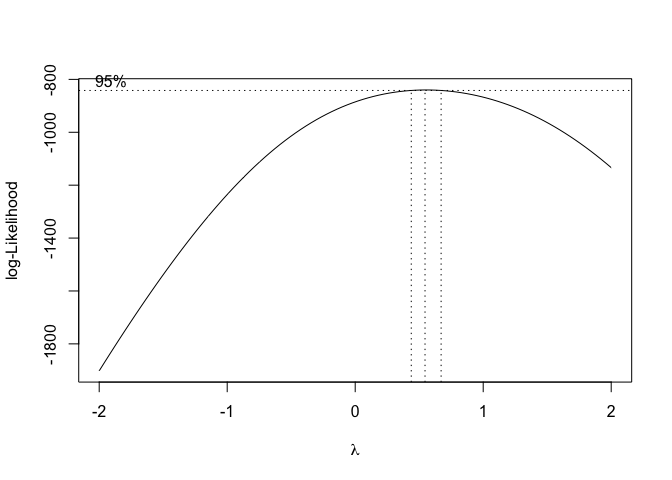
\includegraphics{final_project_files/figure-latex/unnamed-chunk-23-1.pdf}

\begin{Shaded}
\begin{Highlighting}[]
\NormalTok{olsrr}\SpecialCharTok{::}\FunctionTok{ols\_plot\_resid\_qq}\NormalTok{(trans\_fit)}
\end{Highlighting}
\end{Shaded}

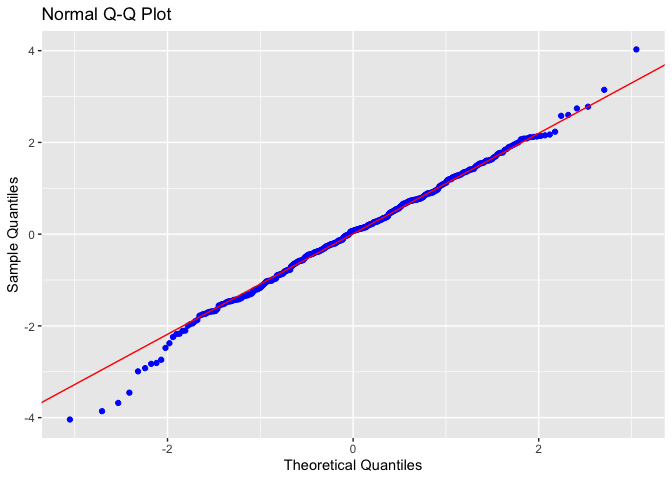
\includegraphics{final_project_files/figure-latex/unnamed-chunk-23-2.pdf}

\begin{Shaded}
\begin{Highlighting}[]
\NormalTok{lambda\_trans }\OtherTok{=}\NormalTok{ MASS}\SpecialCharTok{::}\FunctionTok{boxcox}\NormalTok{(trans\_fit)}
\end{Highlighting}
\end{Shaded}

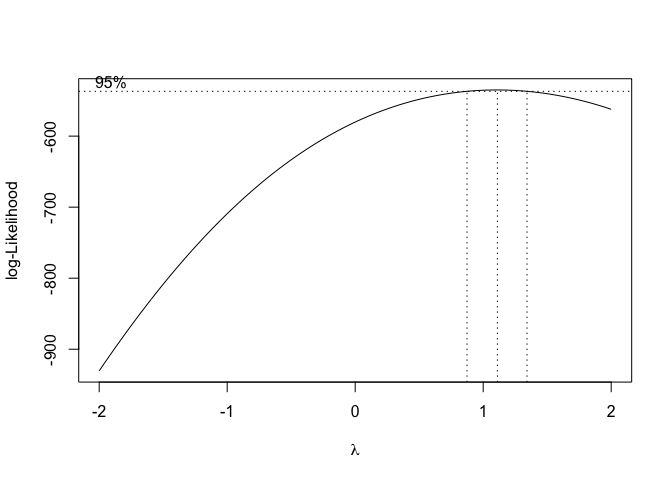
\includegraphics{final_project_files/figure-latex/unnamed-chunk-23-3.pdf}

\begin{Shaded}
\begin{Highlighting}[]
\NormalTok{optlam\_trans }\OtherTok{=}\NormalTok{ lambda\_trans}\SpecialCharTok{$}\NormalTok{x[}\FunctionTok{which.max}\NormalTok{(lambda\_trans}\SpecialCharTok{$}\NormalTok{y)]}
\NormalTok{optlam\_trans}
\end{Highlighting}
\end{Shaded}

\begin{verbatim}
## [1] 1.111111
\end{verbatim}

\hypertarget{counties-with-unusual-rates-1}{%
\subsubsection{Counties with unusual
rates}\label{counties-with-unusual-rates-1}}

\begin{Shaded}
\begin{Highlighting}[]
\NormalTok{upper }\OtherTok{=} \FunctionTok{quantile}\NormalTok{(cdi\_trans}\SpecialCharTok{$}\NormalTok{crm\_1000\_sqr, }\FloatTok{0.75}\NormalTok{)}
\NormalTok{lower }\OtherTok{=} \FunctionTok{quantile}\NormalTok{(cdi\_trans}\SpecialCharTok{$}\NormalTok{crm\_1000\_sqr, }\FloatTok{0.25}\NormalTok{)}
\NormalTok{IQR }\OtherTok{=}\NormalTok{ upper }\SpecialCharTok{{-}}\NormalTok{ lower}

\NormalTok{cdi\_trans }\SpecialCharTok{\%\textgreater{}\%} 
  \FunctionTok{filter}\NormalTok{(crm\_1000\_sqr }\SpecialCharTok{\textgreater{}}\NormalTok{ upper }\SpecialCharTok{+} \FloatTok{1.5}\SpecialCharTok{*}\NormalTok{IQR,}
\NormalTok{         crm\_1000\_sqr }\SpecialCharTok{\textgreater{}}\NormalTok{ lower }\SpecialCharTok{{-}} \FloatTok{1.5}\SpecialCharTok{*}\NormalTok{IQR) }\SpecialCharTok{\%\textgreater{}\%} 
\NormalTok{  dplyr}\SpecialCharTok{::}\FunctionTok{select}\NormalTok{(crm\_1000\_sqr) }\SpecialCharTok{\%\textgreater{}\%} 
  \FunctionTok{mutate}\NormalTok{(}\AttributeTok{cty =} \FunctionTok{c}\NormalTok{(}\StringTok{"Kings"}\NormalTok{, }\StringTok{"St.\_Loui"}\NormalTok{)) }\SpecialCharTok{\%\textgreater{}\%} 
\NormalTok{  knitr}\SpecialCharTok{::}\FunctionTok{kable}\NormalTok{(}\AttributeTok{digits =} \DecValTok{2}\NormalTok{)}
\end{Highlighting}
\end{Shaded}

\begin{longtable}[]{@{}rl@{}}
\toprule
crm\_1000\_sqr & cty \\
\midrule
\endhead
17.20 & Kings \\
12.71 & St.\_Loui \\
\bottomrule
\end{longtable}

\hypertarget{model-selection}{%
\subsection{Model Selection}\label{model-selection}}

\hypertarget{step-wise-approach}{%
\subsubsection{Step-wise approach}\label{step-wise-approach}}

\hypertarget{backward}{%
\paragraph{Backward}\label{backward}}

\begin{Shaded}
\begin{Highlighting}[]
\NormalTok{fit\_back }\OtherTok{=} \FunctionTok{step}\NormalTok{(trans\_fit, }\AttributeTok{direction=}\StringTok{\textquotesingle{}backward\textquotesingle{}}\NormalTok{)}
\end{Highlighting}
\end{Shaded}

\begin{verbatim}
## Start:  AIC=153.85
## crm_1000_sqr ~ pop + pop18 + pop65 + hsgrad + bagrad + poverty + 
##     unemp + pcincome + region + pdocs_1000 + pbeds_1000 + density_pop
## 
##               Df Sum of Sq    RSS    AIC
## - pop65        1     0.044 583.09 151.89
## - pdocs_1000   1     0.451 583.49 152.19
## - unemp        1     2.081 585.12 153.42
## <none>                     583.04 153.85
## - bagrad       1     4.331 587.37 155.11
## - hsgrad       1     5.303 588.35 155.84
## - pop18        1    11.591 594.63 160.51
## - pcincome     1    13.004 596.05 161.56
## - pop          1    16.690 599.73 164.27
## - pbeds_1000   1    22.604 605.65 168.59
## - poverty      1    30.154 613.20 174.04
## - density_pop  1    71.185 654.23 202.54
## - region       3   205.212 788.25 280.54
## 
## Step:  AIC=151.89
## crm_1000_sqr ~ pop + pop18 + hsgrad + bagrad + poverty + unemp + 
##     pcincome + region + pdocs_1000 + pbeds_1000 + density_pop
## 
##               Df Sum of Sq    RSS    AIC
## - pdocs_1000   1     0.446 583.53 150.22
## - unemp        1     2.038 585.12 151.42
## <none>                     583.09 151.89
## - bagrad       1     4.334 587.42 153.15
## - hsgrad       1     5.380 588.47 153.93
## - pcincome     1    13.159 596.25 159.71
## - pop18        1    16.404 599.49 162.09
## - pop          1    16.651 599.74 162.28
## - pbeds_1000   1    23.989 607.08 167.63
## - poverty      1    31.904 614.99 173.33
## - density_pop  1    71.276 654.36 200.63
## - region       3   205.335 788.42 278.63
## 
## Step:  AIC=150.22
## crm_1000_sqr ~ pop + pop18 + hsgrad + bagrad + poverty + unemp + 
##     pcincome + region + pbeds_1000 + density_pop
## 
##               Df Sum of Sq    RSS    AIC
## - unemp        1     2.006 585.54 149.73
## <none>                     583.53 150.22
## - bagrad       1     5.378 588.91 152.26
## - hsgrad       1     5.671 589.20 152.48
## - pcincome     1    12.753 596.29 157.74
## - pop18        1    16.012 599.54 160.13
## - pop          1    16.517 600.05 160.50
## - poverty      1    32.264 615.80 171.90
## - pbeds_1000   1    41.083 624.62 178.16
## - density_pop  1    70.863 654.40 198.65
## - region       3   204.905 788.44 276.64
## 
## Step:  AIC=149.73
## crm_1000_sqr ~ pop + pop18 + hsgrad + bagrad + poverty + pcincome + 
##     region + pbeds_1000 + density_pop
## 
##               Df Sum of Sq    RSS    AIC
## <none>                     585.54 149.73
## - hsgrad       1     4.640 590.18 151.21
## - bagrad       1     7.070 592.61 153.01
## - pcincome     1    15.076 600.61 158.92
## - pop18        1    15.967 601.50 159.57
## - pop          1    16.046 601.58 159.63
## - pbeds_1000   1    39.273 624.81 176.30
## - poverty      1    41.161 626.70 177.62
## - density_pop  1    70.118 655.66 197.50
## - region       3   209.818 795.36 278.49
\end{verbatim}

\begin{Shaded}
\begin{Highlighting}[]
\NormalTok{fit\_back}
\end{Highlighting}
\end{Shaded}

\begin{verbatim}
## 
## Call:
## lm(formula = crm_1000_sqr ~ pop + pop18 + hsgrad + bagrad + poverty + 
##     pcincome + region + pbeds_1000 + density_pop, data = cdi_trans)
## 
## Coefficients:
##        (Intercept)                 pop               pop18              hsgrad  
##         -1.132e+00           3.546e-07           6.390e-02           3.180e-02  
##             bagrad             poverty            pcincome  regionnorthcentral  
##         -4.210e-02           1.298e-01           1.005e-04           6.887e-01  
##        regionsouth          regionwest          pbeds_1000         density_pop  
##          1.933e+00           1.642e+00           1.767e-01           2.117e-04
\end{verbatim}

\begin{Shaded}
\begin{Highlighting}[]
\NormalTok{olsrr}\SpecialCharTok{::}\FunctionTok{ols\_plot\_resid\_fit}\NormalTok{(fit\_back)}
\end{Highlighting}
\end{Shaded}

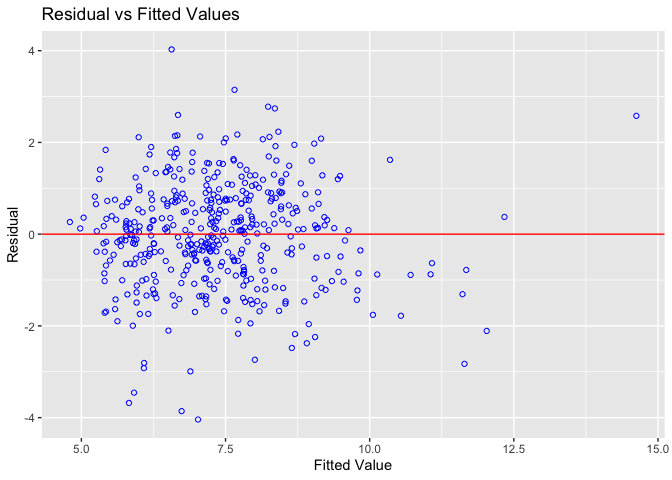
\includegraphics{final_project_files/figure-latex/unnamed-chunk-25-1.pdf}

\begin{Shaded}
\begin{Highlighting}[]
\NormalTok{olsrr}\SpecialCharTok{::}\FunctionTok{ols\_plot\_resid\_qq}\NormalTok{(fit\_back)}
\end{Highlighting}
\end{Shaded}

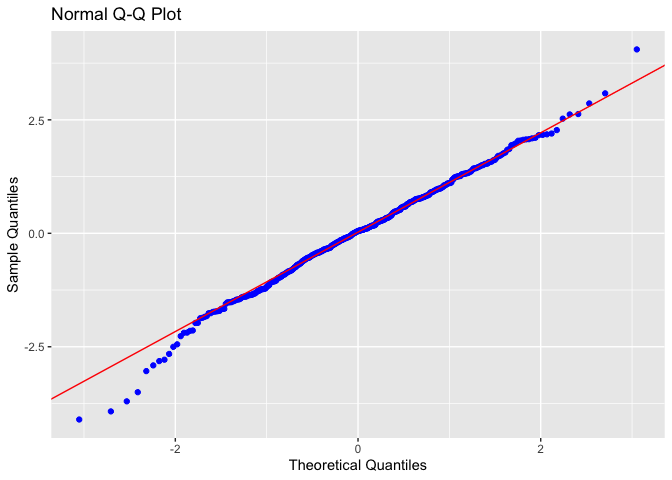
\includegraphics{final_project_files/figure-latex/unnamed-chunk-25-2.pdf}

\begin{Shaded}
\begin{Highlighting}[]
\NormalTok{MASS}\SpecialCharTok{::}\FunctionTok{boxcox}\NormalTok{(fit\_back)}
\end{Highlighting}
\end{Shaded}

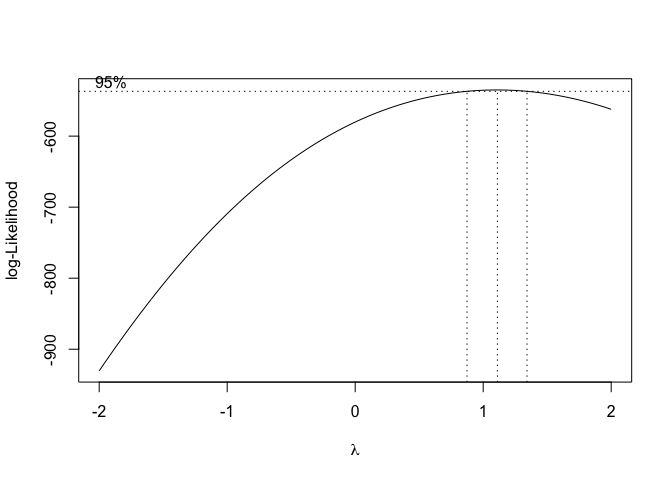
\includegraphics{final_project_files/figure-latex/unnamed-chunk-25-3.pdf}

Backward: crm\_1000\_sqr \textasciitilde{} pop + pop18 + hsgrad + bagrad
+ poverty + pcincome + region + pbeds\_1000 + density\_pop

\hypertarget{forward}{%
\paragraph{forward}\label{forward}}

\begin{Shaded}
\begin{Highlighting}[]
\NormalTok{fit\_forward }\OtherTok{=} \FunctionTok{step}\NormalTok{(trans\_fit, }\AttributeTok{direction=}\StringTok{"forward"}\NormalTok{)}
\end{Highlighting}
\end{Shaded}

\begin{verbatim}
## Start:  AIC=153.85
## crm_1000_sqr ~ pop + pop18 + pop65 + hsgrad + bagrad + poverty + 
##     unemp + pcincome + region + pdocs_1000 + pbeds_1000 + density_pop
\end{verbatim}

\begin{Shaded}
\begin{Highlighting}[]
\NormalTok{fit\_forward}
\end{Highlighting}
\end{Shaded}

\begin{verbatim}
## 
## Call:
## lm(formula = crm_1000_sqr ~ pop + pop18 + pop65 + hsgrad + bagrad + 
##     poverty + unemp + pcincome + region + pdocs_1000 + pbeds_1000 + 
##     density_pop, data = cdi_trans)
## 
## Coefficients:
##        (Intercept)                 pop               pop18               pop65  
##         -1.645e+00           3.624e-07           6.320e-02          -3.609e-03  
##             hsgrad              bagrad             poverty               unemp  
##          3.479e-02          -3.472e-02           1.192e-01           4.305e-02  
##           pcincome  regionnorthcentral         regionsouth          regionwest  
##          9.589e-05           7.062e-01           1.996e+00           1.674e+00  
##         pdocs_1000          pbeds_1000         density_pop  
##         -3.845e-02           2.120e-01           2.150e-04
\end{verbatim}

\begin{Shaded}
\begin{Highlighting}[]
\NormalTok{olsrr}\SpecialCharTok{::}\FunctionTok{ols\_plot\_resid\_fit}\NormalTok{(fit\_forward)}
\end{Highlighting}
\end{Shaded}

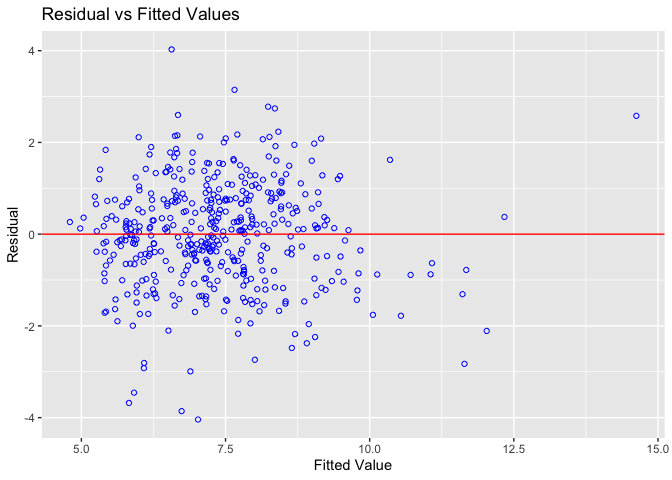
\includegraphics{final_project_files/figure-latex/unnamed-chunk-26-1.pdf}

\begin{Shaded}
\begin{Highlighting}[]
\NormalTok{olsrr}\SpecialCharTok{::}\FunctionTok{ols\_plot\_resid\_qq}\NormalTok{(fit\_forward)}
\end{Highlighting}
\end{Shaded}

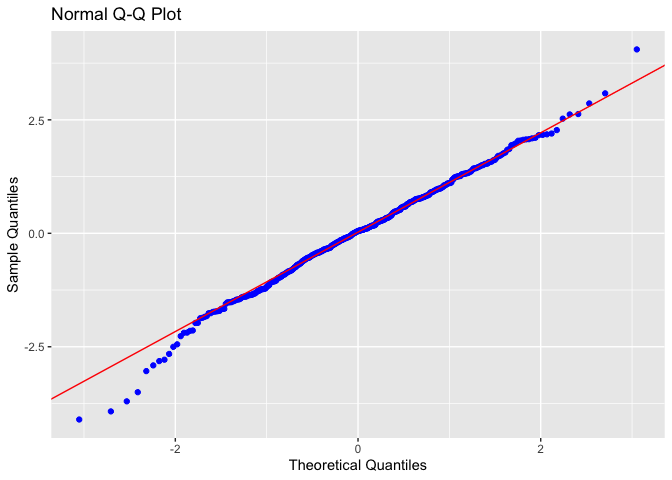
\includegraphics{final_project_files/figure-latex/unnamed-chunk-26-2.pdf}

\begin{Shaded}
\begin{Highlighting}[]
\NormalTok{MASS}\SpecialCharTok{::}\FunctionTok{boxcox}\NormalTok{(fit\_forward)}
\end{Highlighting}
\end{Shaded}

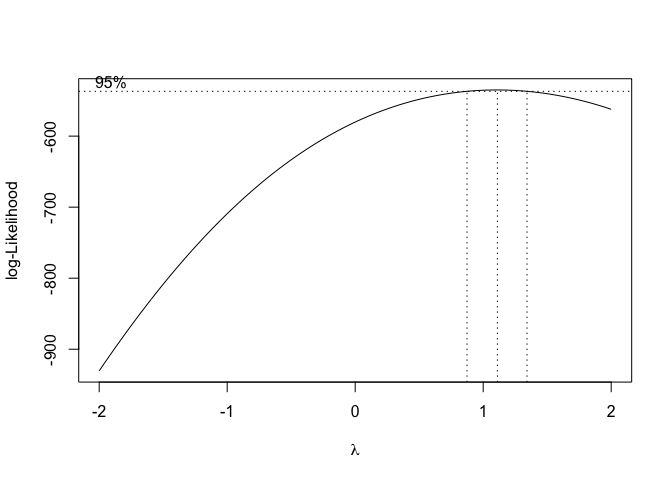
\includegraphics{final_project_files/figure-latex/unnamed-chunk-26-3.pdf}

model: crm\_1000\_sqr \textasciitilde{} pop + pop18 + pop65 + hsgrad +
bagrad + poverty + unemp + pcincome + region + pdocs\_1000 + pbeds\_1000
+ density\_pop, data = cdi\_trans)

\hypertarget{both}{%
\paragraph{both}\label{both}}

step-wise

\begin{Shaded}
\begin{Highlighting}[]
\NormalTok{fit\_both }\OtherTok{=} \FunctionTok{step}\NormalTok{(trans\_fit, }\AttributeTok{direction=}\StringTok{\textquotesingle{}both\textquotesingle{}}\NormalTok{)}
\end{Highlighting}
\end{Shaded}

\begin{verbatim}
## Start:  AIC=153.85
## crm_1000_sqr ~ pop + pop18 + pop65 + hsgrad + bagrad + poverty + 
##     unemp + pcincome + region + pdocs_1000 + pbeds_1000 + density_pop
## 
##               Df Sum of Sq    RSS    AIC
## - pop65        1     0.044 583.09 151.89
## - pdocs_1000   1     0.451 583.49 152.19
## - unemp        1     2.081 585.12 153.42
## <none>                     583.04 153.85
## - bagrad       1     4.331 587.37 155.11
## - hsgrad       1     5.303 588.35 155.84
## - pop18        1    11.591 594.63 160.51
## - pcincome     1    13.004 596.05 161.56
## - pop          1    16.690 599.73 164.27
## - pbeds_1000   1    22.604 605.65 168.59
## - poverty      1    30.154 613.20 174.04
## - density_pop  1    71.185 654.23 202.54
## - region       3   205.212 788.25 280.54
## 
## Step:  AIC=151.89
## crm_1000_sqr ~ pop + pop18 + hsgrad + bagrad + poverty + unemp + 
##     pcincome + region + pdocs_1000 + pbeds_1000 + density_pop
## 
##               Df Sum of Sq    RSS    AIC
## - pdocs_1000   1     0.446 583.53 150.22
## - unemp        1     2.038 585.12 151.42
## <none>                     583.09 151.89
## - bagrad       1     4.334 587.42 153.15
## + pop65        1     0.044 583.04 153.85
## - hsgrad       1     5.380 588.47 153.93
## - pcincome     1    13.159 596.25 159.71
## - pop18        1    16.404 599.49 162.09
## - pop          1    16.651 599.74 162.28
## - pbeds_1000   1    23.989 607.08 167.63
## - poverty      1    31.904 614.99 173.33
## - density_pop  1    71.276 654.36 200.63
## - region       3   205.335 788.42 278.63
## 
## Step:  AIC=150.22
## crm_1000_sqr ~ pop + pop18 + hsgrad + bagrad + poverty + unemp + 
##     pcincome + region + pbeds_1000 + density_pop
## 
##               Df Sum of Sq    RSS    AIC
## - unemp        1     2.006 585.54 149.73
## <none>                     583.53 150.22
## + pdocs_1000   1     0.446 583.09 151.89
## + pop65        1     0.039 583.49 152.19
## - bagrad       1     5.378 588.91 152.26
## - hsgrad       1     5.671 589.20 152.48
## - pcincome     1    12.753 596.29 157.74
## - pop18        1    16.012 599.54 160.13
## - pop          1    16.517 600.05 160.50
## - poverty      1    32.264 615.80 171.90
## - pbeds_1000   1    41.083 624.62 178.16
## - density_pop  1    70.863 654.40 198.65
## - region       3   204.905 788.44 276.64
## 
## Step:  AIC=149.73
## crm_1000_sqr ~ pop + pop18 + hsgrad + bagrad + poverty + pcincome + 
##     region + pbeds_1000 + density_pop
## 
##               Df Sum of Sq    RSS    AIC
## <none>                     585.54 149.73
## + unemp        1     2.006 583.53 150.22
## - hsgrad       1     4.640 590.18 151.21
## + pdocs_1000   1     0.414 585.12 151.42
## + pop65        1     0.000 585.54 151.73
## - bagrad       1     7.070 592.61 153.01
## - pcincome     1    15.076 600.61 158.92
## - pop18        1    15.967 601.50 159.57
## - pop          1    16.046 601.58 159.63
## - pbeds_1000   1    39.273 624.81 176.30
## - poverty      1    41.161 626.70 177.62
## - density_pop  1    70.118 655.66 197.50
## - region       3   209.818 795.36 278.49
\end{verbatim}

\begin{Shaded}
\begin{Highlighting}[]
\NormalTok{fit\_both}
\end{Highlighting}
\end{Shaded}

\begin{verbatim}
## 
## Call:
## lm(formula = crm_1000_sqr ~ pop + pop18 + hsgrad + bagrad + poverty + 
##     pcincome + region + pbeds_1000 + density_pop, data = cdi_trans)
## 
## Coefficients:
##        (Intercept)                 pop               pop18              hsgrad  
##         -1.132e+00           3.546e-07           6.390e-02           3.180e-02  
##             bagrad             poverty            pcincome  regionnorthcentral  
##         -4.210e-02           1.298e-01           1.005e-04           6.887e-01  
##        regionsouth          regionwest          pbeds_1000         density_pop  
##          1.933e+00           1.642e+00           1.767e-01           2.117e-04
\end{verbatim}

lm(formula = crm\_1000\^{}0.5 \textasciitilde{} pop + pop18 + hsgrad +
bagrad + poverty + pcincome + region + pbeds\_1000 + density\_pop, data
= cdi\_model)

This gives back the same model as back

\hypertarget{criterion-based-adjr2-and-cp}{%
\subsubsection{Criterion Based: Adjr2 and
Cp}\label{criterion-based-adjr2-and-cp}}

\begin{Shaded}
\begin{Highlighting}[]
\CommentTok{\# printing the 2 best models of each size. For example, the first two lines: print the best 2 models that have 2 variables (including intercept)}

\NormalTok{models }\OtherTok{\textless{}{-}} \FunctionTok{regsubsets}\NormalTok{(crm\_1000\_sqr }\SpecialCharTok{\textasciitilde{}}\NormalTok{., }\AttributeTok{data =}\NormalTok{ cdi\_trans,}\AttributeTok{nvmax =} \DecValTok{12}\NormalTok{)}
\NormalTok{res\_sum }\OtherTok{=} \FunctionTok{summary}\NormalTok{(models)}

\FunctionTok{par}\NormalTok{(}\AttributeTok{mfrow=}\FunctionTok{c}\NormalTok{(}\DecValTok{1}\NormalTok{,}\DecValTok{2}\NormalTok{))}
\FunctionTok{plot}\NormalTok{(}\DecValTok{1}\SpecialCharTok{:}\DecValTok{12}\NormalTok{, res\_sum}\SpecialCharTok{$}\NormalTok{cp, }\AttributeTok{xlab=}\StringTok{"No of parameters"}\NormalTok{, }\AttributeTok{ylab=}\StringTok{"Cp Statistic"}\NormalTok{)}
\FunctionTok{plot}\NormalTok{(}\DecValTok{1}\SpecialCharTok{:}\DecValTok{12}\NormalTok{, res\_sum}\SpecialCharTok{$}\NormalTok{adjr2, }\AttributeTok{xlab=}\StringTok{"No of parameters"}\NormalTok{, }\AttributeTok{ylab=}\StringTok{"Adj R2"}\NormalTok{)}
\end{Highlighting}
\end{Shaded}

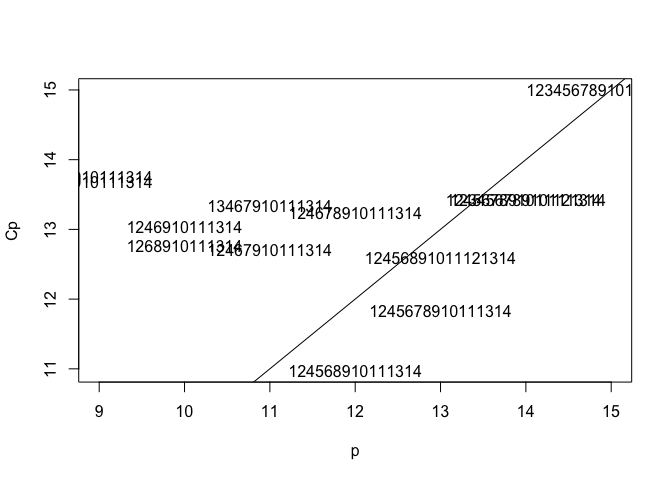
\includegraphics{final_project_files/figure-latex/unnamed-chunk-28-1.pdf}

\begin{Shaded}
\begin{Highlighting}[]
\NormalTok{mod\_s }\OtherTok{=} \FunctionTok{data.frame}\NormalTok{(}
  \AttributeTok{Adj.R2 =} \FunctionTok{which.max}\NormalTok{(res\_sum}\SpecialCharTok{$}\NormalTok{adjr2),}
  \AttributeTok{CP =} \FunctionTok{which.min}\NormalTok{(res\_sum}\SpecialCharTok{$}\NormalTok{cp)}
\NormalTok{)}

\NormalTok{get\_model\_formula }\OtherTok{\textless{}{-}} \ControlFlowTok{function}\NormalTok{(id, object, outcome)\{}
  \CommentTok{\# get models data}
\NormalTok{  models }\OtherTok{\textless{}{-}} \FunctionTok{summary}\NormalTok{(object)}\SpecialCharTok{$}\NormalTok{which[id,}\SpecialCharTok{{-}}\DecValTok{1}\NormalTok{]}
  \CommentTok{\# Get outcome variable}
  \CommentTok{\#form \textless{}{-} as.formula(object$call[[2]])}
  \CommentTok{\#outcome \textless{}{-} all.vars(form)[1]}
  \CommentTok{\# Get model predictors}
\NormalTok{  predictors }\OtherTok{\textless{}{-}} \FunctionTok{names}\NormalTok{(}\FunctionTok{which}\NormalTok{(models }\SpecialCharTok{==} \ConstantTok{TRUE}\NormalTok{))}
\NormalTok{  predictors }\OtherTok{\textless{}{-}} \FunctionTok{paste}\NormalTok{(predictors, }\AttributeTok{collapse =} \StringTok{"+"}\NormalTok{)}
  \CommentTok{\# Build model formula}
  \FunctionTok{as.formula}\NormalTok{(}\FunctionTok{paste0}\NormalTok{(outcome, }\StringTok{"\textasciitilde{}"}\NormalTok{, predictors))}
\NormalTok{\}}
\end{Highlighting}
\end{Shaded}

Model chosen by Adj \(R^2\):

\begin{Shaded}
\begin{Highlighting}[]
\FunctionTok{get\_model\_formula}\NormalTok{(}\DecValTok{12}\NormalTok{, models, }\StringTok{"crm\_1000\_sqr"}\NormalTok{)}
\end{Highlighting}
\end{Shaded}

\begin{verbatim}
## crm_1000_sqr ~ pop + pop18 + hsgrad + bagrad + poverty + unemp + 
##     pcincome + regionnorthcentral + regionsouth + regionwest + 
##     pbeds_1000 + density_pop
## <environment: 0x7fed56451768>
\end{verbatim}

\begin{Shaded}
\begin{Highlighting}[]
\NormalTok{fit\_adjr }\OtherTok{=} \FunctionTok{lm}\NormalTok{(crm\_1000\_sqr }\SpecialCharTok{\textasciitilde{}}\NormalTok{ pop }\SpecialCharTok{+}\NormalTok{ pop18 }\SpecialCharTok{+}\NormalTok{ hsgrad }\SpecialCharTok{+}\NormalTok{ bagrad }\SpecialCharTok{+}\NormalTok{ poverty }\SpecialCharTok{+}\NormalTok{ unemp }\SpecialCharTok{+}\NormalTok{ pcincome }\SpecialCharTok{+}\NormalTok{ region}\SpecialCharTok{+}\NormalTok{ pbeds\_1000 }\SpecialCharTok{+}\NormalTok{ density\_pop, }\AttributeTok{data =}\NormalTok{ cdi\_trans)}

\NormalTok{olsrr}\SpecialCharTok{::}\FunctionTok{ols\_plot\_resid\_fit}\NormalTok{(fit\_adjr)}
\end{Highlighting}
\end{Shaded}

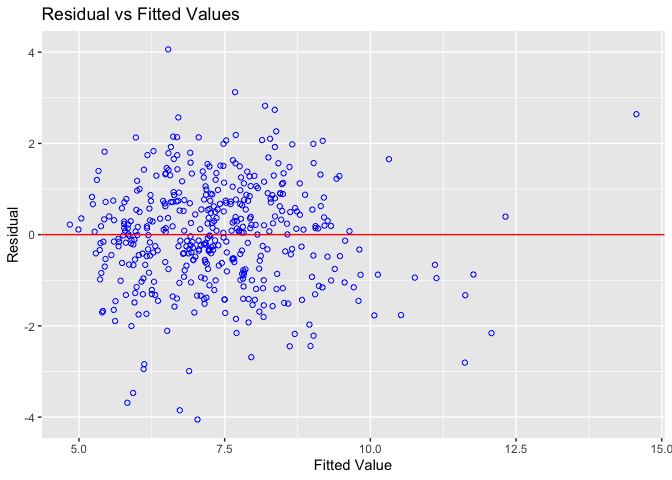
\includegraphics{final_project_files/figure-latex/unnamed-chunk-30-1.pdf}

\begin{Shaded}
\begin{Highlighting}[]
\NormalTok{olsrr}\SpecialCharTok{::}\FunctionTok{ols\_plot\_resid\_qq}\NormalTok{(fit\_adjr)}
\end{Highlighting}
\end{Shaded}

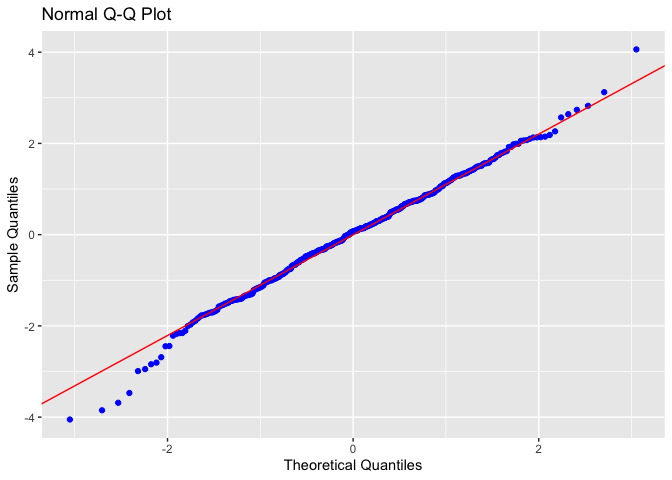
\includegraphics{final_project_files/figure-latex/unnamed-chunk-30-2.pdf}

\begin{Shaded}
\begin{Highlighting}[]
\NormalTok{MASS}\SpecialCharTok{::}\FunctionTok{boxcox}\NormalTok{(fit\_adjr)}
\end{Highlighting}
\end{Shaded}

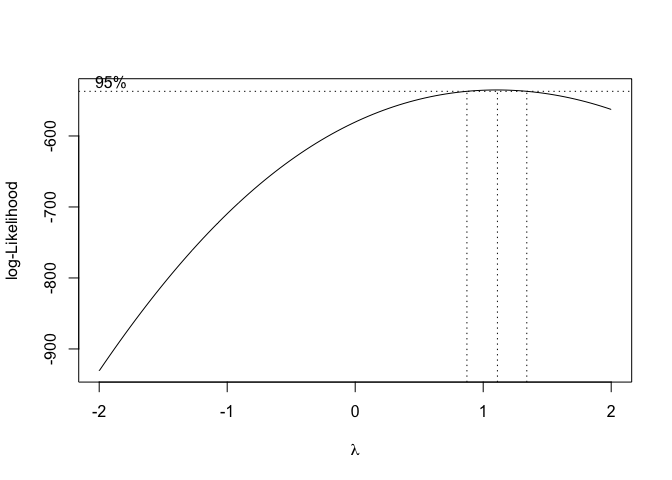
\includegraphics{final_project_files/figure-latex/unnamed-chunk-30-3.pdf}

crm\_1000\_sqr \textasciitilde{} pop + pop18 + hsgrad + bagrad + poverty
+ unemp + pcincome + region+ pbeds\_1000 + density\_pop

Model chosen by Cp: Same with backward

\begin{Shaded}
\begin{Highlighting}[]
\FunctionTok{get\_model\_formula}\NormalTok{(}\DecValTok{11}\NormalTok{, models, }\StringTok{"crm\_1000\_sqr"}\NormalTok{)}
\end{Highlighting}
\end{Shaded}

\begin{verbatim}
## crm_1000_sqr ~ pop + pop18 + hsgrad + bagrad + poverty + pcincome + 
##     regionnorthcentral + regionsouth + regionwest + pbeds_1000 + 
##     density_pop
## <environment: 0x7fed562f93b0>
\end{verbatim}

crm\_1000\_sqr \textasciitilde{} pop + pop18 + hsgrad + bagrad + poverty
+ pcincome + region+ pbeds\_1000 + density\_pop

\begin{Shaded}
\begin{Highlighting}[]
\NormalTok{fit\_Cp }\OtherTok{=} \FunctionTok{lm}\NormalTok{(crm\_1000\_sqr }\SpecialCharTok{\textasciitilde{}}\NormalTok{ pop }\SpecialCharTok{+}\NormalTok{ pop18 }\SpecialCharTok{+}\NormalTok{ hsgrad }\SpecialCharTok{+}\NormalTok{ bagrad }\SpecialCharTok{+}\NormalTok{ poverty }\SpecialCharTok{+}\NormalTok{ pcincome }\SpecialCharTok{+}\NormalTok{ region}\SpecialCharTok{+}\NormalTok{ pbeds\_1000 }\SpecialCharTok{+}\NormalTok{ density\_pop, }\AttributeTok{data=}\NormalTok{cdi\_trans)}

\NormalTok{olsrr}\SpecialCharTok{::}\FunctionTok{ols\_plot\_resid\_fit}\NormalTok{(fit\_Cp)}
\end{Highlighting}
\end{Shaded}

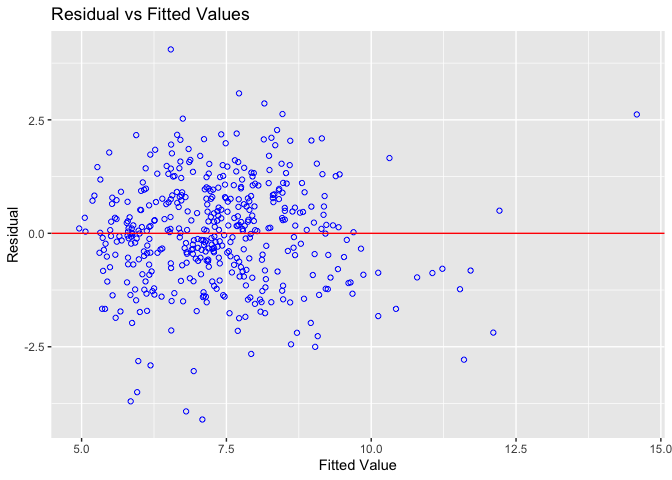
\includegraphics{final_project_files/figure-latex/unnamed-chunk-32-1.pdf}

\begin{Shaded}
\begin{Highlighting}[]
\NormalTok{olsrr}\SpecialCharTok{::}\FunctionTok{ols\_plot\_resid\_qq}\NormalTok{(fit\_Cp)}
\end{Highlighting}
\end{Shaded}

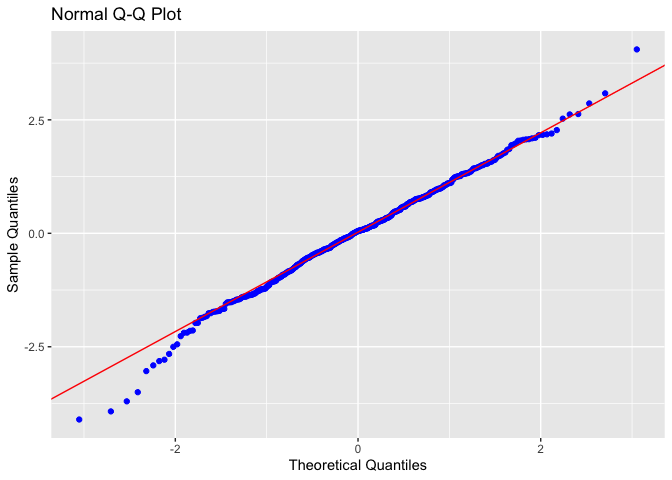
\includegraphics{final_project_files/figure-latex/unnamed-chunk-32-2.pdf}

\begin{Shaded}
\begin{Highlighting}[]
\NormalTok{MASS}\SpecialCharTok{::}\FunctionTok{boxcox}\NormalTok{(fit\_Cp)}
\end{Highlighting}
\end{Shaded}

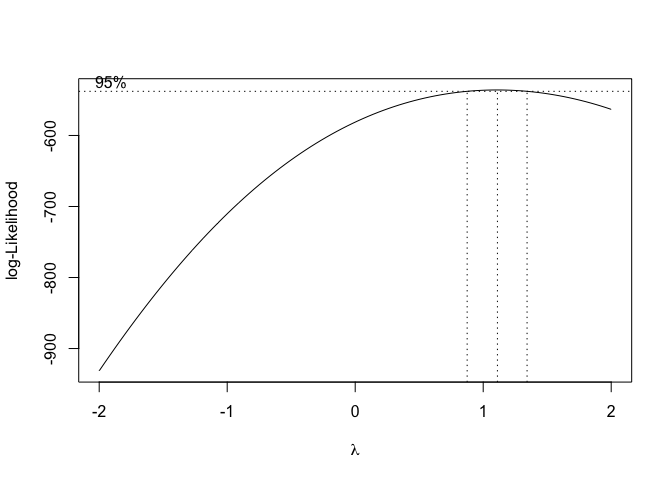
\includegraphics{final_project_files/figure-latex/unnamed-chunk-32-3.pdf}

\hypertarget{check-collinearity}{%
\subsection{Check Collinearity}\label{check-collinearity}}

\begin{Shaded}
\begin{Highlighting}[]
\NormalTok{performance}\SpecialCharTok{::}\FunctionTok{check\_collinearity}\NormalTok{(fit\_back)}
\end{Highlighting}
\end{Shaded}

\begin{verbatim}
## # Check for Multicollinearity
## 
## Low Correlation
## 
##         Term  VIF Increased SE Tolerance
##          pop 1.00         1.00      1.00
##        pop18 1.93         1.39      0.52
##       hsgrad 3.15         1.78      0.32
##       bagrad 3.35         1.83      0.30
##      poverty 2.16         1.47      0.46
##     pcincome 1.03         1.01      0.97
##       region 1.63         1.28      0.61
##   pbeds_1000 1.32         1.15      0.76
##  density_pop 1.01         1.00      0.99
\end{verbatim}

\begin{Shaded}
\begin{Highlighting}[]
\NormalTok{performance}\SpecialCharTok{::}\FunctionTok{check\_collinearity}\NormalTok{(fit\_forward)}
\end{Highlighting}
\end{Shaded}

\begin{verbatim}
## # Check for Multicollinearity
## 
## Low Correlation
## 
##         Term  VIF Increased SE Tolerance
##          pop 1.00         1.00      1.00
##        pop18 2.60         1.61      0.38
##        pop65 2.05         1.43      0.49
##       hsgrad 3.30         1.82      0.30
##       bagrad 3.72         1.93      0.27
##      poverty 2.48         1.58      0.40
##        unemp 1.89         1.37      0.53
##     pcincome 1.02         1.01      0.98
##       region 1.99         1.41      0.50
##   pdocs_1000 2.75         1.66      0.36
##   pbeds_1000 3.31         1.82      0.30
##  density_pop 1.00         1.00      1.00
\end{verbatim}

\begin{Shaded}
\begin{Highlighting}[]
\NormalTok{performance}\SpecialCharTok{::}\FunctionTok{check\_collinearity}\NormalTok{(fit\_adjr)}
\end{Highlighting}
\end{Shaded}

\begin{verbatim}
## # Check for Multicollinearity
## 
## Low Correlation
## 
##         Term  VIF Increased SE Tolerance
##          pop 1.00         1.00      1.00
##        pop18 1.93         1.39      0.52
##       hsgrad 3.27         1.81      0.31
##       bagrad 3.49         1.87      0.29
##      poverty 2.38         1.54      0.42
##        unemp 1.86         1.36      0.54
##     pcincome 1.03         1.01      0.97
##       region 1.83         1.35      0.55
##   pbeds_1000 1.44         1.20      0.69
##  density_pop 1.00         1.00      1.00
\end{verbatim}

\begin{Shaded}
\begin{Highlighting}[]
\NormalTok{performance}\SpecialCharTok{::}\FunctionTok{check\_collinearity}\NormalTok{(fit\_Cp)}
\end{Highlighting}
\end{Shaded}

\begin{verbatim}
## # Check for Multicollinearity
## 
## Low Correlation
## 
##         Term  VIF Increased SE Tolerance
##          pop 1.00         1.00      1.00
##        pop18 1.93         1.39      0.52
##       hsgrad 3.15         1.78      0.32
##       bagrad 3.35         1.83      0.30
##      poverty 2.16         1.47      0.46
##     pcincome 1.03         1.01      0.97
##       region 1.63         1.28      0.61
##   pbeds_1000 1.32         1.15      0.76
##  density_pop 1.01         1.00      0.99
\end{verbatim}

Delete predictors when vif larger than 10. Non of them are greater than
10. So all of the models are good, don't have to worry about
collinearity.

\hypertarget{checking-to-outliers-and-influential-points}{%
\subsection{Checking to Outliers and Influential
Points}\label{checking-to-outliers-and-influential-points}}

\begin{Shaded}
\begin{Highlighting}[]
\NormalTok{olsrr}\SpecialCharTok{::}\FunctionTok{ols\_plot\_cooksd\_bar}\NormalTok{(fit\_back, }\AttributeTok{print\_plot =} \ConstantTok{TRUE}\NormalTok{)}
\end{Highlighting}
\end{Shaded}

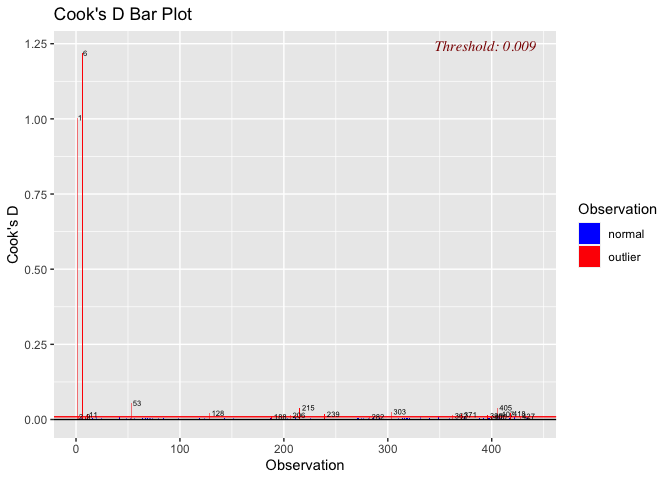
\includegraphics{final_project_files/figure-latex/unnamed-chunk-34-1.pdf}

\begin{Shaded}
\begin{Highlighting}[]
\CommentTok{\#remove observations whose cook\textquotesingle{}s D \textgreater{} 0.5}
\NormalTok{cdi\_trans\_without }\OtherTok{=}\NormalTok{ cdi\_trans[}\SpecialCharTok{{-}}\FunctionTok{c}\NormalTok{(}\DecValTok{1}\NormalTok{, }\DecValTok{6}\NormalTok{),]}
\end{Highlighting}
\end{Shaded}

\hypertarget{build-model-without-outlier}{%
\subsection{Build model without
outlier}\label{build-model-without-outlier}}

Built the without model with \textbf{fit\_back}

\begin{Shaded}
\begin{Highlighting}[]
\NormalTok{fit\_back\_without }\OtherTok{=} \FunctionTok{lm}\NormalTok{(crm\_1000\_sqr }\SpecialCharTok{\textasciitilde{}}\NormalTok{ pop }\SpecialCharTok{+}\NormalTok{ pop18 }\SpecialCharTok{+}\NormalTok{ hsgrad }\SpecialCharTok{+}\NormalTok{ bagrad }\SpecialCharTok{+}\NormalTok{ poverty }\SpecialCharTok{+}\NormalTok{ pcincome }\SpecialCharTok{+}\NormalTok{ region }\SpecialCharTok{+}\NormalTok{ pbeds\_1000 }\SpecialCharTok{+}\NormalTok{ density\_pop, }\AttributeTok{data =}\NormalTok{ cdi\_trans\_without)}

\FunctionTok{summary}\NormalTok{(fit\_back\_without)}
\end{Highlighting}
\end{Shaded}

\begin{verbatim}
## 
## Call:
## lm(formula = crm_1000_sqr ~ pop + pop18 + hsgrad + bagrad + poverty + 
##     pcincome + region + pbeds_1000 + density_pop, data = cdi_trans_without)
## 
## Residuals:
##     Min      1Q  Median      3Q     Max 
## -4.1228 -0.6365  0.0530  0.7450  3.9171 
## 
## Coefficients:
##                      Estimate Std. Error t value Pr(>|t|)    
## (Intercept)        -9.873e-01  1.576e+00  -0.626 0.531435    
## pop                 7.169e-07  1.419e-07   5.053 6.46e-07 ***
## pop18               7.526e-02  1.855e-02   4.056 5.93e-05 ***
## hsgrad              2.185e-02  1.695e-02   1.289 0.198159    
## bagrad             -4.136e-02  1.808e-02  -2.288 0.022652 *  
## poverty             1.219e-01  2.319e-02   5.254 2.35e-07 ***
## pcincome            1.121e-04  3.068e-05   3.655 0.000289 ***
## regionnorthcentral  7.058e-01  1.702e-01   4.146 4.08e-05 ***
## regionsouth         1.951e+00  1.617e-01  12.066  < 2e-16 ***
## regionwest          1.691e+00  1.971e-01   8.579  < 2e-16 ***
## pbeds_1000          2.036e-01  3.274e-02   6.217 1.21e-09 ***
## density_pop         7.859e-05  4.288e-05   1.833 0.067561 .  
## ---
## Signif. codes:  0 '***' 0.001 '**' 0.01 '*' 0.05 '.' 0.1 ' ' 1
## 
## Residual standard error: 1.14 on 426 degrees of freedom
## Multiple R-squared:  0.5488, Adjusted R-squared:  0.5372 
## F-statistic: 47.11 on 11 and 426 DF,  p-value: < 2.2e-16
\end{verbatim}

\begin{Shaded}
\begin{Highlighting}[]
\CommentTok{\# Residual performance}
\FunctionTok{par}\NormalTok{(}\AttributeTok{mfrow=}\FunctionTok{c}\NormalTok{(}\DecValTok{2}\NormalTok{,}\DecValTok{2}\NormalTok{))}
\NormalTok{olsrr}\SpecialCharTok{::}\FunctionTok{ols\_plot\_resid\_fit}\NormalTok{(fit\_back\_without)}
\end{Highlighting}
\end{Shaded}

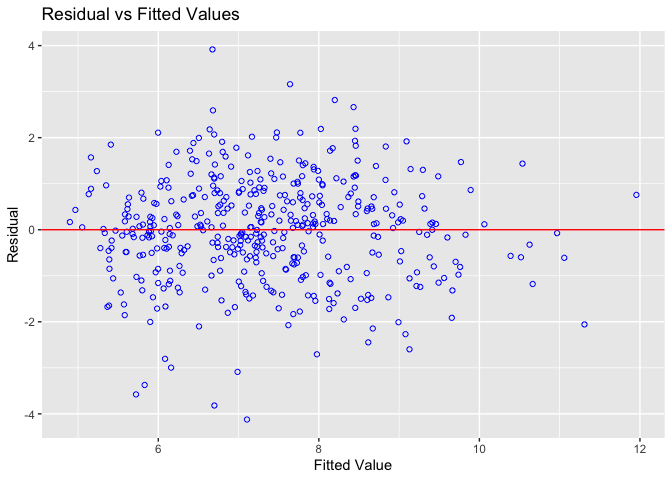
\includegraphics{final_project_files/figure-latex/unnamed-chunk-35-1.pdf}

\begin{Shaded}
\begin{Highlighting}[]
\NormalTok{olsrr}\SpecialCharTok{::}\FunctionTok{ols\_plot\_resid\_qq}\NormalTok{(fit\_back\_without)}
\end{Highlighting}
\end{Shaded}

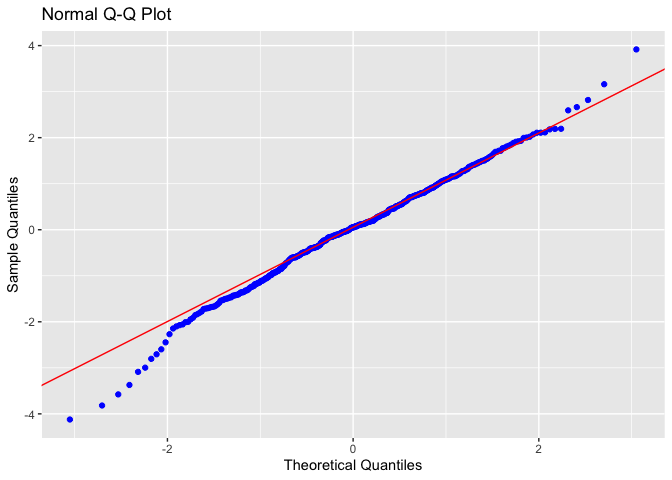
\includegraphics{final_project_files/figure-latex/unnamed-chunk-35-2.pdf}

Build the without model with \textbf{trans\_fit} (full model)

\begin{Shaded}
\begin{Highlighting}[]
\NormalTok{trans\_fit\_without }\OtherTok{=} \FunctionTok{lm}\NormalTok{(crm\_1000\_sqr }\SpecialCharTok{\textasciitilde{}}\NormalTok{., }\AttributeTok{data =}\NormalTok{ cdi\_trans\_without)}

\FunctionTok{summary}\NormalTok{(trans\_fit\_without)}
\end{Highlighting}
\end{Shaded}

\begin{verbatim}
## 
## Call:
## lm(formula = crm_1000_sqr ~ ., data = cdi_trans_without)
## 
## Residuals:
##     Min      1Q  Median      3Q     Max 
## -4.0654 -0.6625  0.0540  0.7183  3.9085 
## 
## Coefficients:
##                      Estimate Std. Error t value Pr(>|t|)    
## (Intercept)        -1.643e+00  1.767e+00  -0.930 0.353040    
## pop                 7.281e-07  1.425e-07   5.111 4.87e-07 ***
## pop18               7.584e-02  2.159e-02   3.513 0.000491 ***
## pop65              -2.316e-04  1.965e-02  -0.012 0.990601    
## hsgrad              2.583e-02  1.733e-02   1.491 0.136820    
## bagrad             -3.462e-02  1.911e-02  -1.812 0.070658 .  
## poverty             1.111e-01  2.492e-02   4.457 1.07e-05 ***
## unemp               4.736e-02  3.407e-02   1.390 0.165214    
## pcincome            1.058e-04  3.141e-05   3.367 0.000828 ***
## regionnorthcentral  7.343e-01  1.755e-01   4.184 3.49e-05 ***
## regionsouth         2.024e+00  1.707e-01  11.857  < 2e-16 ***
## regionwest          1.719e+00  2.008e-01   8.565  < 2e-16 ***
## pdocs_1000         -2.102e-02  6.581e-02  -0.319 0.749576    
## pbeds_1000          2.286e-01  5.101e-02   4.481 9.59e-06 ***
## density_pop         8.083e-05  4.359e-05   1.854 0.064417 .  
## ---
## Signif. codes:  0 '***' 0.001 '**' 0.01 '*' 0.05 '.' 0.1 ' ' 1
## 
## Residual standard error: 1.141 on 423 degrees of freedom
## Multiple R-squared:  0.551,  Adjusted R-squared:  0.5361 
## F-statistic: 37.08 on 14 and 423 DF,  p-value: < 2.2e-16
\end{verbatim}

\begin{Shaded}
\begin{Highlighting}[]
\CommentTok{\# Residual performance}
\FunctionTok{par}\NormalTok{(}\AttributeTok{mfrow=}\FunctionTok{c}\NormalTok{(}\DecValTok{2}\NormalTok{,}\DecValTok{2}\NormalTok{))}
\NormalTok{olsrr}\SpecialCharTok{::}\FunctionTok{ols\_plot\_resid\_fit}\NormalTok{(trans\_fit\_without)}
\end{Highlighting}
\end{Shaded}

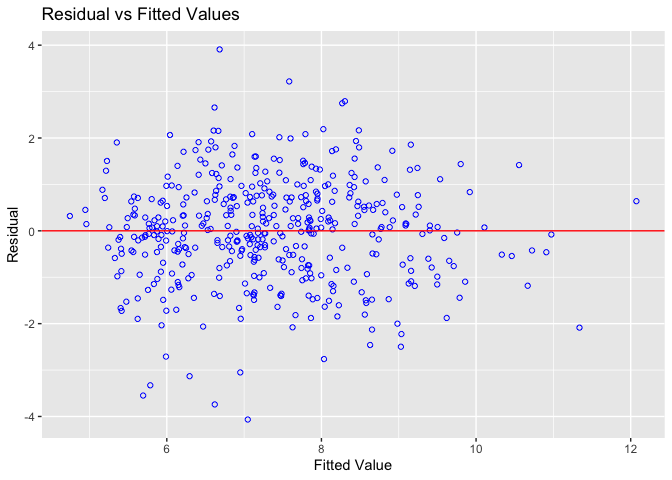
\includegraphics{final_project_files/figure-latex/unnamed-chunk-36-1.pdf}

\begin{Shaded}
\begin{Highlighting}[]
\NormalTok{olsrr}\SpecialCharTok{::}\FunctionTok{ols\_plot\_resid\_qq}\NormalTok{(trans\_fit\_without)}
\end{Highlighting}
\end{Shaded}

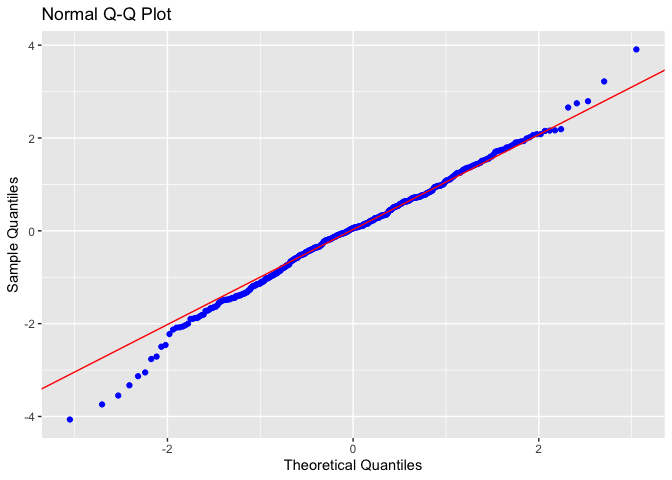
\includegraphics{final_project_files/figure-latex/unnamed-chunk-36-2.pdf}

Built the without model with \textbf{fit\_adjr}

\begin{Shaded}
\begin{Highlighting}[]
\NormalTok{fit\_adjr\_without }\OtherTok{=} \FunctionTok{lm}\NormalTok{(crm\_1000\_sqr }\SpecialCharTok{\textasciitilde{}}\NormalTok{ pop }\SpecialCharTok{+}\NormalTok{ pop18 }\SpecialCharTok{+}\NormalTok{ hsgrad }\SpecialCharTok{+}\NormalTok{ bagrad }\SpecialCharTok{+}\NormalTok{ poverty }\SpecialCharTok{+}\NormalTok{ unemp }\SpecialCharTok{+}\NormalTok{ pcincome }\SpecialCharTok{+}\NormalTok{ region}\SpecialCharTok{+}\NormalTok{ pbeds\_1000 }\SpecialCharTok{+}\NormalTok{ density\_pop, }\AttributeTok{data =}\NormalTok{ cdi\_trans\_without)}

\FunctionTok{summary}\NormalTok{(fit\_adjr\_without)}
\end{Highlighting}
\end{Shaded}

\begin{verbatim}
## 
## Call:
## lm(formula = crm_1000_sqr ~ pop + pop18 + hsgrad + bagrad + poverty + 
##     unemp + pcincome + region + pbeds_1000 + density_pop, data = cdi_trans_without)
## 
## Residuals:
##     Min      1Q  Median      3Q     Max 
## -4.0662 -0.6619  0.0502  0.7174  3.9254 
## 
## Coefficients:
##                      Estimate Std. Error t value Pr(>|t|)    
## (Intercept)        -1.620e+00  1.638e+00  -0.989 0.323424    
## pop                 7.261e-07  1.419e-07   5.118 4.69e-07 ***
## pop18               7.546e-02  1.853e-02   4.072 5.57e-05 ***
## hsgrad              2.624e-02  1.722e-02   1.524 0.128270    
## bagrad             -3.617e-02  1.844e-02  -1.962 0.050439 .  
## poverty             1.115e-01  2.432e-02   4.584 6.01e-06 ***
## unemp               4.714e-02  3.372e-02   1.398 0.162867    
## pcincome            1.048e-04  3.108e-05   3.373 0.000811 ***
## regionnorthcentral  7.374e-01  1.715e-01   4.299 2.13e-05 ***
## regionsouth         2.025e+00  1.700e-01  11.913  < 2e-16 ***
## regionwest          1.711e+00  1.974e-01   8.667  < 2e-16 ***
## pbeds_1000          2.172e-01  3.414e-02   6.363 5.12e-10 ***
## density_pop         7.881e-05  4.283e-05   1.840 0.066502 .  
## ---
## Signif. codes:  0 '***' 0.001 '**' 0.01 '*' 0.05 '.' 0.1 ' ' 1
## 
## Residual standard error: 1.138 on 425 degrees of freedom
## Multiple R-squared:  0.5509, Adjusted R-squared:  0.5382 
## F-statistic: 43.45 on 12 and 425 DF,  p-value: < 2.2e-16
\end{verbatim}

\begin{Shaded}
\begin{Highlighting}[]
\CommentTok{\# Residual performance}
\FunctionTok{par}\NormalTok{(}\AttributeTok{mfrow=}\FunctionTok{c}\NormalTok{(}\DecValTok{2}\NormalTok{,}\DecValTok{2}\NormalTok{))}
\NormalTok{olsrr}\SpecialCharTok{::}\FunctionTok{ols\_plot\_resid\_fit}\NormalTok{(fit\_adjr\_without)}
\end{Highlighting}
\end{Shaded}

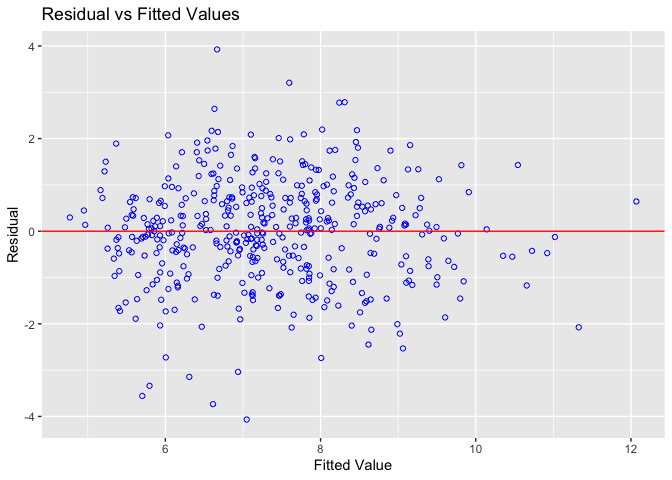
\includegraphics{final_project_files/figure-latex/unnamed-chunk-37-1.pdf}

\begin{Shaded}
\begin{Highlighting}[]
\NormalTok{olsrr}\SpecialCharTok{::}\FunctionTok{ols\_plot\_resid\_qq}\NormalTok{(fit\_adjr\_without)}
\end{Highlighting}
\end{Shaded}

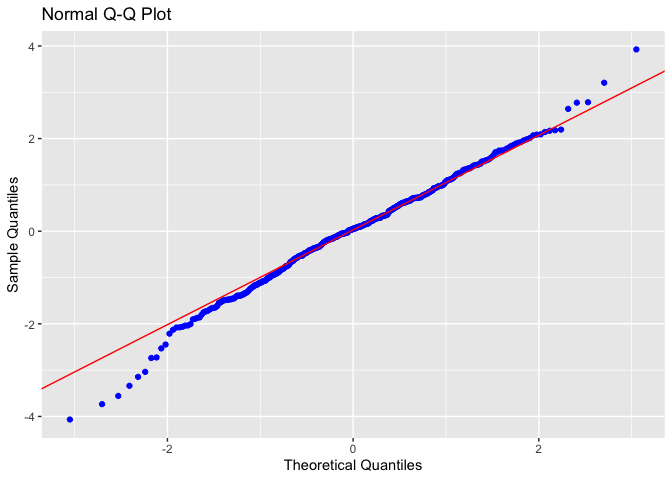
\includegraphics{final_project_files/figure-latex/unnamed-chunk-37-2.pdf}

\hypertarget{criteria}{%
\subsection{Criteria}\label{criteria}}

\hypertarget{cp-for-models-fit-without-outlier}{%
\paragraph{Cp for models fit without
outlier}\label{cp-for-models-fit-without-outlier}}

\begin{Shaded}
\begin{Highlighting}[]
\NormalTok{olsrr}\SpecialCharTok{::}\FunctionTok{ols\_mallows\_cp}\NormalTok{(fit\_back\_without,trans\_fit) }\CommentTok{\#{-}14.65}
\end{Highlighting}
\end{Shaded}

\begin{verbatim}
## [1] -14.65265
\end{verbatim}

\begin{Shaded}
\begin{Highlighting}[]
\NormalTok{olsrr}\SpecialCharTok{::}\FunctionTok{ols\_mallows\_cp}\NormalTok{(trans\_fit\_without,trans\_fit)}\CommentTok{\# {-}10.59}
\end{Highlighting}
\end{Shaded}

\begin{verbatim}
## [1] -10.5956
\end{verbatim}

\begin{Shaded}
\begin{Highlighting}[]
\NormalTok{olsrr}\SpecialCharTok{::}\FunctionTok{ols\_mallows\_cp}\NormalTok{(fit\_adjr\_without,trans\_fit) }\CommentTok{\#{-}14.49}
\end{Highlighting}
\end{Shaded}

\begin{verbatim}
## [1] -14.49878
\end{verbatim}

\hypertarget{aic}{%
\paragraph{AIC}\label{aic}}

\begin{Shaded}
\begin{Highlighting}[]
\FunctionTok{AIC}\NormalTok{(fit\_back\_without) }\CommentTok{\# 1371.373}
\end{Highlighting}
\end{Shaded}

\begin{verbatim}
## [1] 1371.373
\end{verbatim}

\begin{Shaded}
\begin{Highlighting}[]
\FunctionTok{AIC}\NormalTok{(trans\_fit\_without) }\CommentTok{\#1375.258}
\end{Highlighting}
\end{Shaded}

\begin{verbatim}
## [1] 1375.258
\end{verbatim}

\begin{Shaded}
\begin{Highlighting}[]
\FunctionTok{AIC}\NormalTok{(fit\_adjr\_without) }\CommentTok{\# 1371.363}
\end{Highlighting}
\end{Shaded}

\begin{verbatim}
## [1] 1371.363
\end{verbatim}

\hypertarget{bic}{%
\paragraph{BIC}\label{bic}}

\begin{Shaded}
\begin{Highlighting}[]
\FunctionTok{BIC}\NormalTok{(fit\_back\_without) }\CommentTok{\#1424.441}
\end{Highlighting}
\end{Shaded}

\begin{verbatim}
## [1] 1424.441
\end{verbatim}

\begin{Shaded}
\begin{Highlighting}[]
\FunctionTok{BIC}\NormalTok{(trans\_fit\_without) }\CommentTok{\#1440,573}
\end{Highlighting}
\end{Shaded}

\begin{verbatim}
## [1] 1440.573
\end{verbatim}

\begin{Shaded}
\begin{Highlighting}[]
\FunctionTok{BIC}\NormalTok{(fit\_adjr\_without) }\CommentTok{\# 1428.514}
\end{Highlighting}
\end{Shaded}

\begin{verbatim}
## [1] 1428.514
\end{verbatim}

\hypertarget{mse}{%
\paragraph{MSE}\label{mse}}

\begin{Shaded}
\begin{Highlighting}[]
\NormalTok{back\_without\_summ }\OtherTok{=}\FunctionTok{summary}\NormalTok{(fit\_back\_without) }\CommentTok{\#1.2633}
\FunctionTok{mean}\NormalTok{(back\_without\_summ}\SpecialCharTok{$}\NormalTok{residuals}\SpecialCharTok{\^{}}\DecValTok{2}\NormalTok{)}
\end{Highlighting}
\end{Shaded}

\begin{verbatim}
## [1] 1.263328
\end{verbatim}

\begin{Shaded}
\begin{Highlighting}[]
\NormalTok{trans\_without\_summ }\OtherTok{=}\FunctionTok{summary}\NormalTok{(trans\_fit\_without) }\CommentTok{\#1.2572}
\FunctionTok{mean}\NormalTok{(trans\_without\_summ}\SpecialCharTok{$}\NormalTok{residuals}\SpecialCharTok{\^{}}\DecValTok{2}\NormalTok{)}
\end{Highlighting}
\end{Shaded}

\begin{verbatim}
## [1] 1.257243
\end{verbatim}

\begin{Shaded}
\begin{Highlighting}[]
\NormalTok{adjr\_without\_summ }\OtherTok{=}\FunctionTok{summary}\NormalTok{(fit\_adjr\_without) }\CommentTok{\#1.2575}
\FunctionTok{mean}\NormalTok{(adjr\_without\_summ}\SpecialCharTok{$}\NormalTok{residuals}\SpecialCharTok{\^{}}\DecValTok{2}\NormalTok{)}
\end{Highlighting}
\end{Shaded}

\begin{verbatim}
## [1] 1.257546
\end{verbatim}

\hypertarget{model-validation}{%
\section{Model Validation}\label{model-validation}}

\hypertarget{compute-rmse-mspe-adjusted-r2-by-cross-validation}{%
\subsection{Compute RMSE, MSPE, adjusted R\^{}2 by
cross-validation}\label{compute-rmse-mspe-adjusted-r2-by-cross-validation}}

Using back and adjr model and data without outlier

\begin{Shaded}
\begin{Highlighting}[]
\FunctionTok{library}\NormalTok{(modelr)}
\FunctionTok{set.seed}\NormalTok{(}\DecValTok{1}\NormalTok{)}
\NormalTok{cv\_df }\OtherTok{=} 
  \FunctionTok{crossv\_kfold}\NormalTok{(cdi\_trans\_without, }\AttributeTok{k =} \DecValTok{5}\NormalTok{) }\SpecialCharTok{\%\textgreater{}\%} 
  \FunctionTok{mutate}\NormalTok{(}
    \AttributeTok{train =} \FunctionTok{map}\NormalTok{(train, as\_tibble),}
    \AttributeTok{test =} \FunctionTok{map}\NormalTok{(test, as\_tibble))}

\NormalTok{cv\_df }\OtherTok{=} 
\NormalTok{  cv\_df }\SpecialCharTok{\%\textgreater{}\%}
  \FunctionTok{mutate}\NormalTok{(}
    \AttributeTok{fit\_back =} \FunctionTok{map}\NormalTok{(train, }\SpecialCharTok{\textasciitilde{}}\FunctionTok{lm}\NormalTok{(crm\_1000\_sqr }\SpecialCharTok{\textasciitilde{}}\NormalTok{ pop }\SpecialCharTok{+}\NormalTok{ pop18 }\SpecialCharTok{+}\NormalTok{ hsgrad }\SpecialCharTok{+}\NormalTok{ bagrad }\SpecialCharTok{+}\NormalTok{ poverty }\SpecialCharTok{+}\NormalTok{ pcincome }\SpecialCharTok{+}\NormalTok{ region }\SpecialCharTok{+}\NormalTok{ pbeds\_1000 }\SpecialCharTok{+}\NormalTok{ density\_pop, }\AttributeTok{data =}\NormalTok{ .x)),}
    \AttributeTok{trans\_fit =} \FunctionTok{map}\NormalTok{(train, }\SpecialCharTok{\textasciitilde{}}\FunctionTok{lm}\NormalTok{(crm\_1000\_sqr }\SpecialCharTok{\textasciitilde{}}\NormalTok{ pop }\SpecialCharTok{+}\NormalTok{ pop18 }\SpecialCharTok{+}\NormalTok{ pop65}\SpecialCharTok{+}\NormalTok{ hsgrad }\SpecialCharTok{+}\NormalTok{ bagrad }\SpecialCharTok{+}\NormalTok{ poverty }\SpecialCharTok{+}\NormalTok{ unemp }\SpecialCharTok{+}\NormalTok{ pcincome }\SpecialCharTok{+}\NormalTok{ region}\SpecialCharTok{+} \SpecialCharTok{+}\NormalTok{pdocs\_1000}\SpecialCharTok{+}\NormalTok{pbeds\_1000 }\SpecialCharTok{+}\NormalTok{ density\_pop, }\AttributeTok{data =}\NormalTok{ .x)),}
    \AttributeTok{fit\_adjr =} \FunctionTok{map}\NormalTok{(train, }\SpecialCharTok{\textasciitilde{}}\FunctionTok{lm}\NormalTok{(crm\_1000\_sqr }\SpecialCharTok{\textasciitilde{}}\NormalTok{ pop }\SpecialCharTok{+}\NormalTok{ pop18 }\SpecialCharTok{+}\NormalTok{ hsgrad }\SpecialCharTok{+}\NormalTok{ bagrad }\SpecialCharTok{+}\NormalTok{ poverty }\SpecialCharTok{+}\NormalTok{ unemp }\SpecialCharTok{+}\NormalTok{ pcincome }\SpecialCharTok{+}\NormalTok{ region}\SpecialCharTok{+}\NormalTok{ pbeds\_1000 }\SpecialCharTok{+}\NormalTok{ density\_pop, }\AttributeTok{data =}\NormalTok{ .x))) }\SpecialCharTok{\%\textgreater{}\%} 
  \FunctionTok{mutate}\NormalTok{(}
    \AttributeTok{rmse\_back =} \FunctionTok{map2\_dbl}\NormalTok{(fit\_back, test, }\SpecialCharTok{\textasciitilde{}}\FunctionTok{rmse}\NormalTok{(}\AttributeTok{model =}\NormalTok{ .x, }\AttributeTok{data =}\NormalTok{ .y)),}
    \AttributeTok{rmse\_full =} \FunctionTok{map2\_dbl}\NormalTok{(trans\_fit, test, }\SpecialCharTok{\textasciitilde{}}\FunctionTok{rmse}\NormalTok{(}\AttributeTok{model =}\NormalTok{ .x, }\AttributeTok{data =}\NormalTok{ .y)),}
    \AttributeTok{rmse\_adjr =} \FunctionTok{map2\_dbl}\NormalTok{(fit\_adjr, test, }\SpecialCharTok{\textasciitilde{}}\FunctionTok{rmse}\NormalTok{(}\AttributeTok{model =}\NormalTok{ .x, }\AttributeTok{data =}\NormalTok{ .y))) }\SpecialCharTok{\%\textgreater{}\%}
  \FunctionTok{mutate}\NormalTok{(}
    \AttributeTok{mspe\_back =} \FunctionTok{map2\_dbl}\NormalTok{(fit\_back, test, }\SpecialCharTok{\textasciitilde{}} \FunctionTok{mean}\NormalTok{((.y}\SpecialCharTok{$}\NormalTok{crm\_1000\_sqr }\SpecialCharTok{{-}}\FunctionTok{predict.lm}\NormalTok{(.x,.y))}\SpecialCharTok{\^{}}\DecValTok{2}\NormalTok{)),}
    \AttributeTok{mspe\_full =} \FunctionTok{map2\_dbl}\NormalTok{(trans\_fit, test, }\SpecialCharTok{\textasciitilde{}} \FunctionTok{mean}\NormalTok{((.y}\SpecialCharTok{$}\NormalTok{crm\_1000\_sqr }\SpecialCharTok{{-}}\FunctionTok{predict.lm}\NormalTok{(.x,.y))}\SpecialCharTok{\^{}}\DecValTok{2}\NormalTok{)),}
    \AttributeTok{mspe\_adjr =} \FunctionTok{map2\_dbl}\NormalTok{(fit\_adjr, test, }\SpecialCharTok{\textasciitilde{}} \FunctionTok{mean}\NormalTok{((.y}\SpecialCharTok{$}\NormalTok{crm\_1000\_sqr }\SpecialCharTok{{-}}\FunctionTok{predict.lm}\NormalTok{(.x,.y))}\SpecialCharTok{\^{}}\DecValTok{2}\NormalTok{))) }\SpecialCharTok{\%\textgreater{}\%} 
  \FunctionTok{mutate}\NormalTok{(}
    \AttributeTok{res\_back =} \FunctionTok{map}\NormalTok{(fit\_back, broom}\SpecialCharTok{::}\NormalTok{glance }\SpecialCharTok{\%\textgreater{}\%}\NormalTok{ as.data.frame),}
    \AttributeTok{res\_full =} \FunctionTok{map}\NormalTok{(trans\_fit, broom}\SpecialCharTok{::}\NormalTok{glance }\SpecialCharTok{\%\textgreater{}\%}\NormalTok{ as.data.frame),}
    \AttributeTok{res\_adjr =} \FunctionTok{map}\NormalTok{(fit\_adjr, broom}\SpecialCharTok{::}\NormalTok{glance }\SpecialCharTok{\%\textgreater{}\%}\NormalTok{ as.data.frame)) }\SpecialCharTok{\%\textgreater{}\%}
  \FunctionTok{unnest}\NormalTok{(res\_back, res\_full, res\_adjr) }\SpecialCharTok{\%\textgreater{}\%}
\NormalTok{  dplyr}\SpecialCharTok{::}\FunctionTok{select}\NormalTok{(rmse\_back,rmse\_full,rmse\_adjr,}
\NormalTok{                mspe\_back,mspe\_full,mspe\_adjr,}
\NormalTok{                value.adj.r.squared,value.adj.r.squared1,value.adj.r.squared2) }\SpecialCharTok{\%\textgreater{}\%}
  \FunctionTok{rename}\NormalTok{(}\AttributeTok{adjR\_back =}\NormalTok{ value.adj.r.squared,}
         \AttributeTok{adjR\_full =}\NormalTok{ value.adj.r.squared1,}
         \AttributeTok{adjR\_adjr =}\NormalTok{ value.adj.r.squared2)}

\NormalTok{cv\_df }\SpecialCharTok{\%\textgreater{}\%}
  \FunctionTok{summarise\_each}\NormalTok{(}\FunctionTok{funs}\NormalTok{(}\FunctionTok{mean}\NormalTok{( .,}\AttributeTok{na.rm =} \ConstantTok{TRUE}\NormalTok{))) }\SpecialCharTok{\%\textgreater{}\%}
  \FunctionTok{t}\NormalTok{()}
\end{Highlighting}
\end{Shaded}

\begin{verbatim}
##                [,1]
## rmse_back 1.1675477
## rmse_full 1.1812447
## rmse_adjr 1.1656535
## mspe_back 1.3695900
## mspe_full 1.4017130
## mspe_adjr 1.3651876
## adjR_back 0.5378246
## adjR_full 0.5371541
## adjR_adjr 0.5386250
\end{verbatim}

\hypertarget{plot-the-violin-plot}{%
\subsection{Plot the violin plot}\label{plot-the-violin-plot}}

\begin{Shaded}
\begin{Highlighting}[]
\NormalTok{unnest\_cd\_df }\OtherTok{=}\NormalTok{ cv\_df }\SpecialCharTok{\%\textgreater{}\%}
  \FunctionTok{pivot\_longer}\NormalTok{(rmse\_back}\SpecialCharTok{:}\NormalTok{adjR\_adjr, }
               \AttributeTok{names\_pattern =} \StringTok{"(.*)(....)$"}\NormalTok{, }
               \AttributeTok{names\_to =} \FunctionTok{c}\NormalTok{(}\StringTok{"limit"}\NormalTok{, }\StringTok{"model"}\NormalTok{)) }\SpecialCharTok{\%\textgreater{}\%} 
  \FunctionTok{mutate}\NormalTok{(}\AttributeTok{limit=}\FunctionTok{ifelse}\NormalTok{(limit}\SpecialCharTok{==}\StringTok{""}\NormalTok{, }\StringTok{"value"}\NormalTok{, limit)) }\SpecialCharTok{\%\textgreater{}\%}
  \FunctionTok{pivot\_wider}\NormalTok{(}\AttributeTok{id\_cols =}\NormalTok{ model, }
              \AttributeTok{names\_from =}\NormalTok{ limit, }
              \AttributeTok{values\_from =}\NormalTok{ value, }
              \AttributeTok{names\_repair =} \StringTok{"check\_unique"}\NormalTok{) }\SpecialCharTok{\%\textgreater{}\%} 
  \FunctionTok{unnest}\NormalTok{(}\FunctionTok{c}\NormalTok{(rmse\_, adjR\_)) }\SpecialCharTok{\%\textgreater{}\%}
  \FunctionTok{rename}\NormalTok{(}\AttributeTok{rmse =}\NormalTok{ rmse\_,}
         \AttributeTok{adjR =}\NormalTok{ adjR\_)}
\NormalTok{unnest\_cd\_df }\SpecialCharTok{\%\textgreater{}\%} \FunctionTok{ggplot}\NormalTok{(}\FunctionTok{aes}\NormalTok{(}\AttributeTok{x =}\NormalTok{ model, }\AttributeTok{y =}\NormalTok{ rmse)) }\SpecialCharTok{+} \FunctionTok{geom\_violin}\NormalTok{() }
\end{Highlighting}
\end{Shaded}

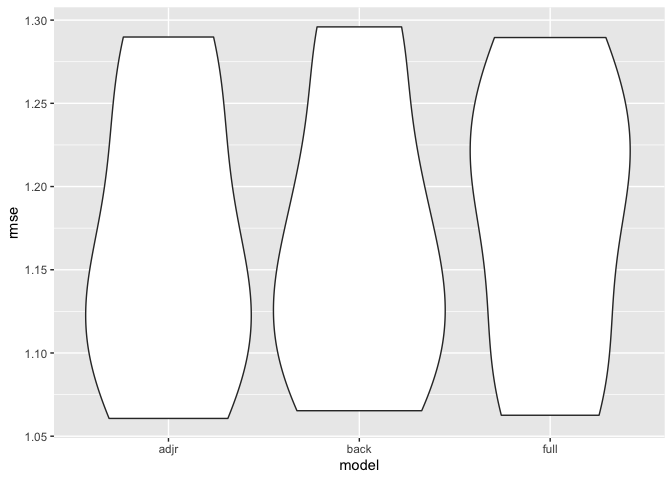
\includegraphics{final_project_files/figure-latex/unnamed-chunk-43-1.pdf}

\begin{Shaded}
\begin{Highlighting}[]
\NormalTok{unnest\_cd\_df }\SpecialCharTok{\%\textgreater{}\%} \FunctionTok{ggplot}\NormalTok{(}\FunctionTok{aes}\NormalTok{(}\AttributeTok{x =}\NormalTok{ model, }\AttributeTok{y =}\NormalTok{ adjR)) }\SpecialCharTok{+} \FunctionTok{geom\_violin}\NormalTok{() }
\end{Highlighting}
\end{Shaded}

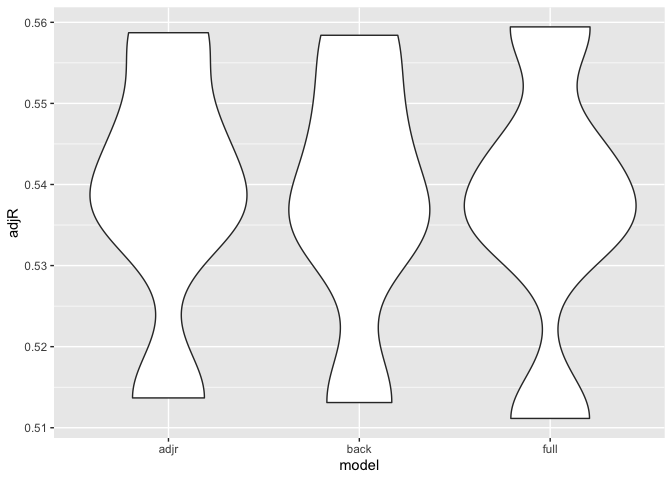
\includegraphics{final_project_files/figure-latex/unnamed-chunk-43-2.pdf}

\end{document}
